\newpage
\chapter{Smart Grid: Architettura e componenti}

\section{Introduzione alla Smart Grid}

%  altri possono essere:
% Il Dominio Fisico della Smart Grid: Struttura e Componenti Fondamentali // consigliato
% Anatomia della Rete Elettrica Intelligente
% La Transizione Energetica e l'Architettura della Smart Grid
% L'Architettura della Smart Grid: dalla Produzione al Consumo



Il paradigma energetico contemporaneo è caratterizzato da una trasformazione radicale, spinta dalla crescente integrazione di Fonti Energetiche Rinnovabili (FER). Tale transizione ha favorito la proliferazione della generazione distribuita (DER): impianti di piccola taglia, spesso di proprietà degli stessi consumatori, che immettono energia in rete. Questa dinamica trasforma il ruolo del consumatore passivo in quello di \textit{Prosumer}\footnote{\textit{Prosumer}: Unione di \textit{Consumer} (consumatore) e \textit{Producer} (Produttore)}, un attore attivo capace sia di consumare che di produrre energia. \label{prosumer}



Di conseguenza, il modello tradizionale di flusso energetico, storicamente monodirezionale dalla centrale all'utente, è stato soppiantato da un modello complesso e bidirezionale \cite{Enel}. In questo scenario, la rete elettrica tradizionale mostra i propri limiti strutturali. La risposta a questa sfida è la Smart Grid, o Rete Intelligente: un'evoluzione dell'infrastruttura elettrica che, integrando tecnologie avanzate di sensoristica, comunicazione e controllo, è progettata per gestire i flussi energetici in modo efficiente, sicuro e resiliente \cite{en15186799}.





% Una \textbf{Smart Grid}, o Rete Intelligente, è l'evoluzione della tradizionale rete elettrica. Si basa su componenti avanzati di \textbf{rilevamento}, \textbf{comunicazione} e \textbf{decisione} per ottenere una trasmissione e distribuzione di energia \textbf{sicura}, \textbf{efficiente} e \textbf{resiliente}. \cite{en15186799}


% L'aumento di anno in anno di fonti rinnovabili ha portato ad una crescita significativa della generazione di energia distribuita, chiamata anche Distributed Energy Resources (DER), ovvero la produzione di energia tramite piccoli impianti connessi alla rete di distribuzione elettrica posseduti dai Consumatori-Produttori o Posumers\footnote{Prosumer: Unione di Consumer (consumatori) e Producer (Produttori)}. 


% In questo contesto di flussi non più monodirezionali, bensì bidirezionali, l'utilizzo di Smart Grid può essere di grande aiuto per le aziende di Trasmissione e Distribuzione dell'energia elettrica. \cite{Enel}


% \begin{figure}[h!]
%     \centering
%     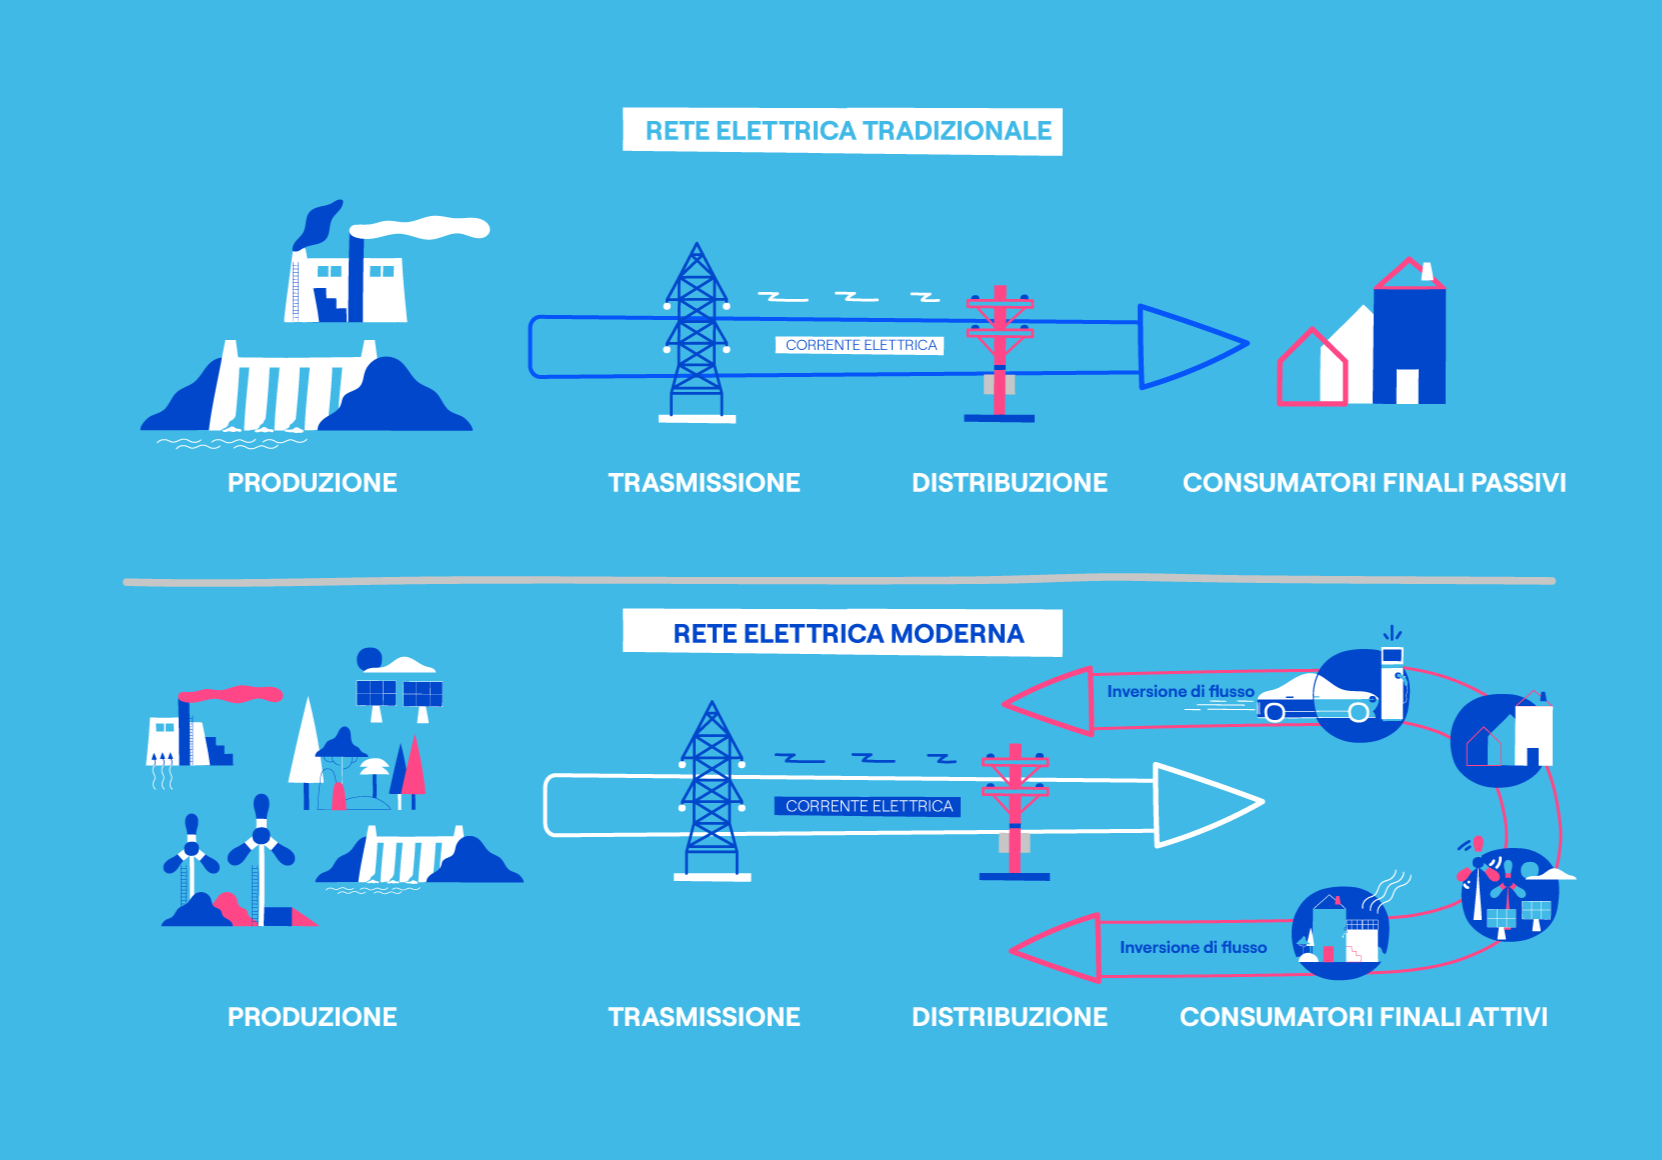
\includegraphics[width=0.8\linewidth]{img/Smart-Grid-EDistribuzione2.png}
%     \caption{Confronto rete tradizionale e rete intelligente}
%     \label{fig:TraditionalGridVSSmartrGrid}
% \end{figure}


% \begin{figure}[h!]
%     \centering
%     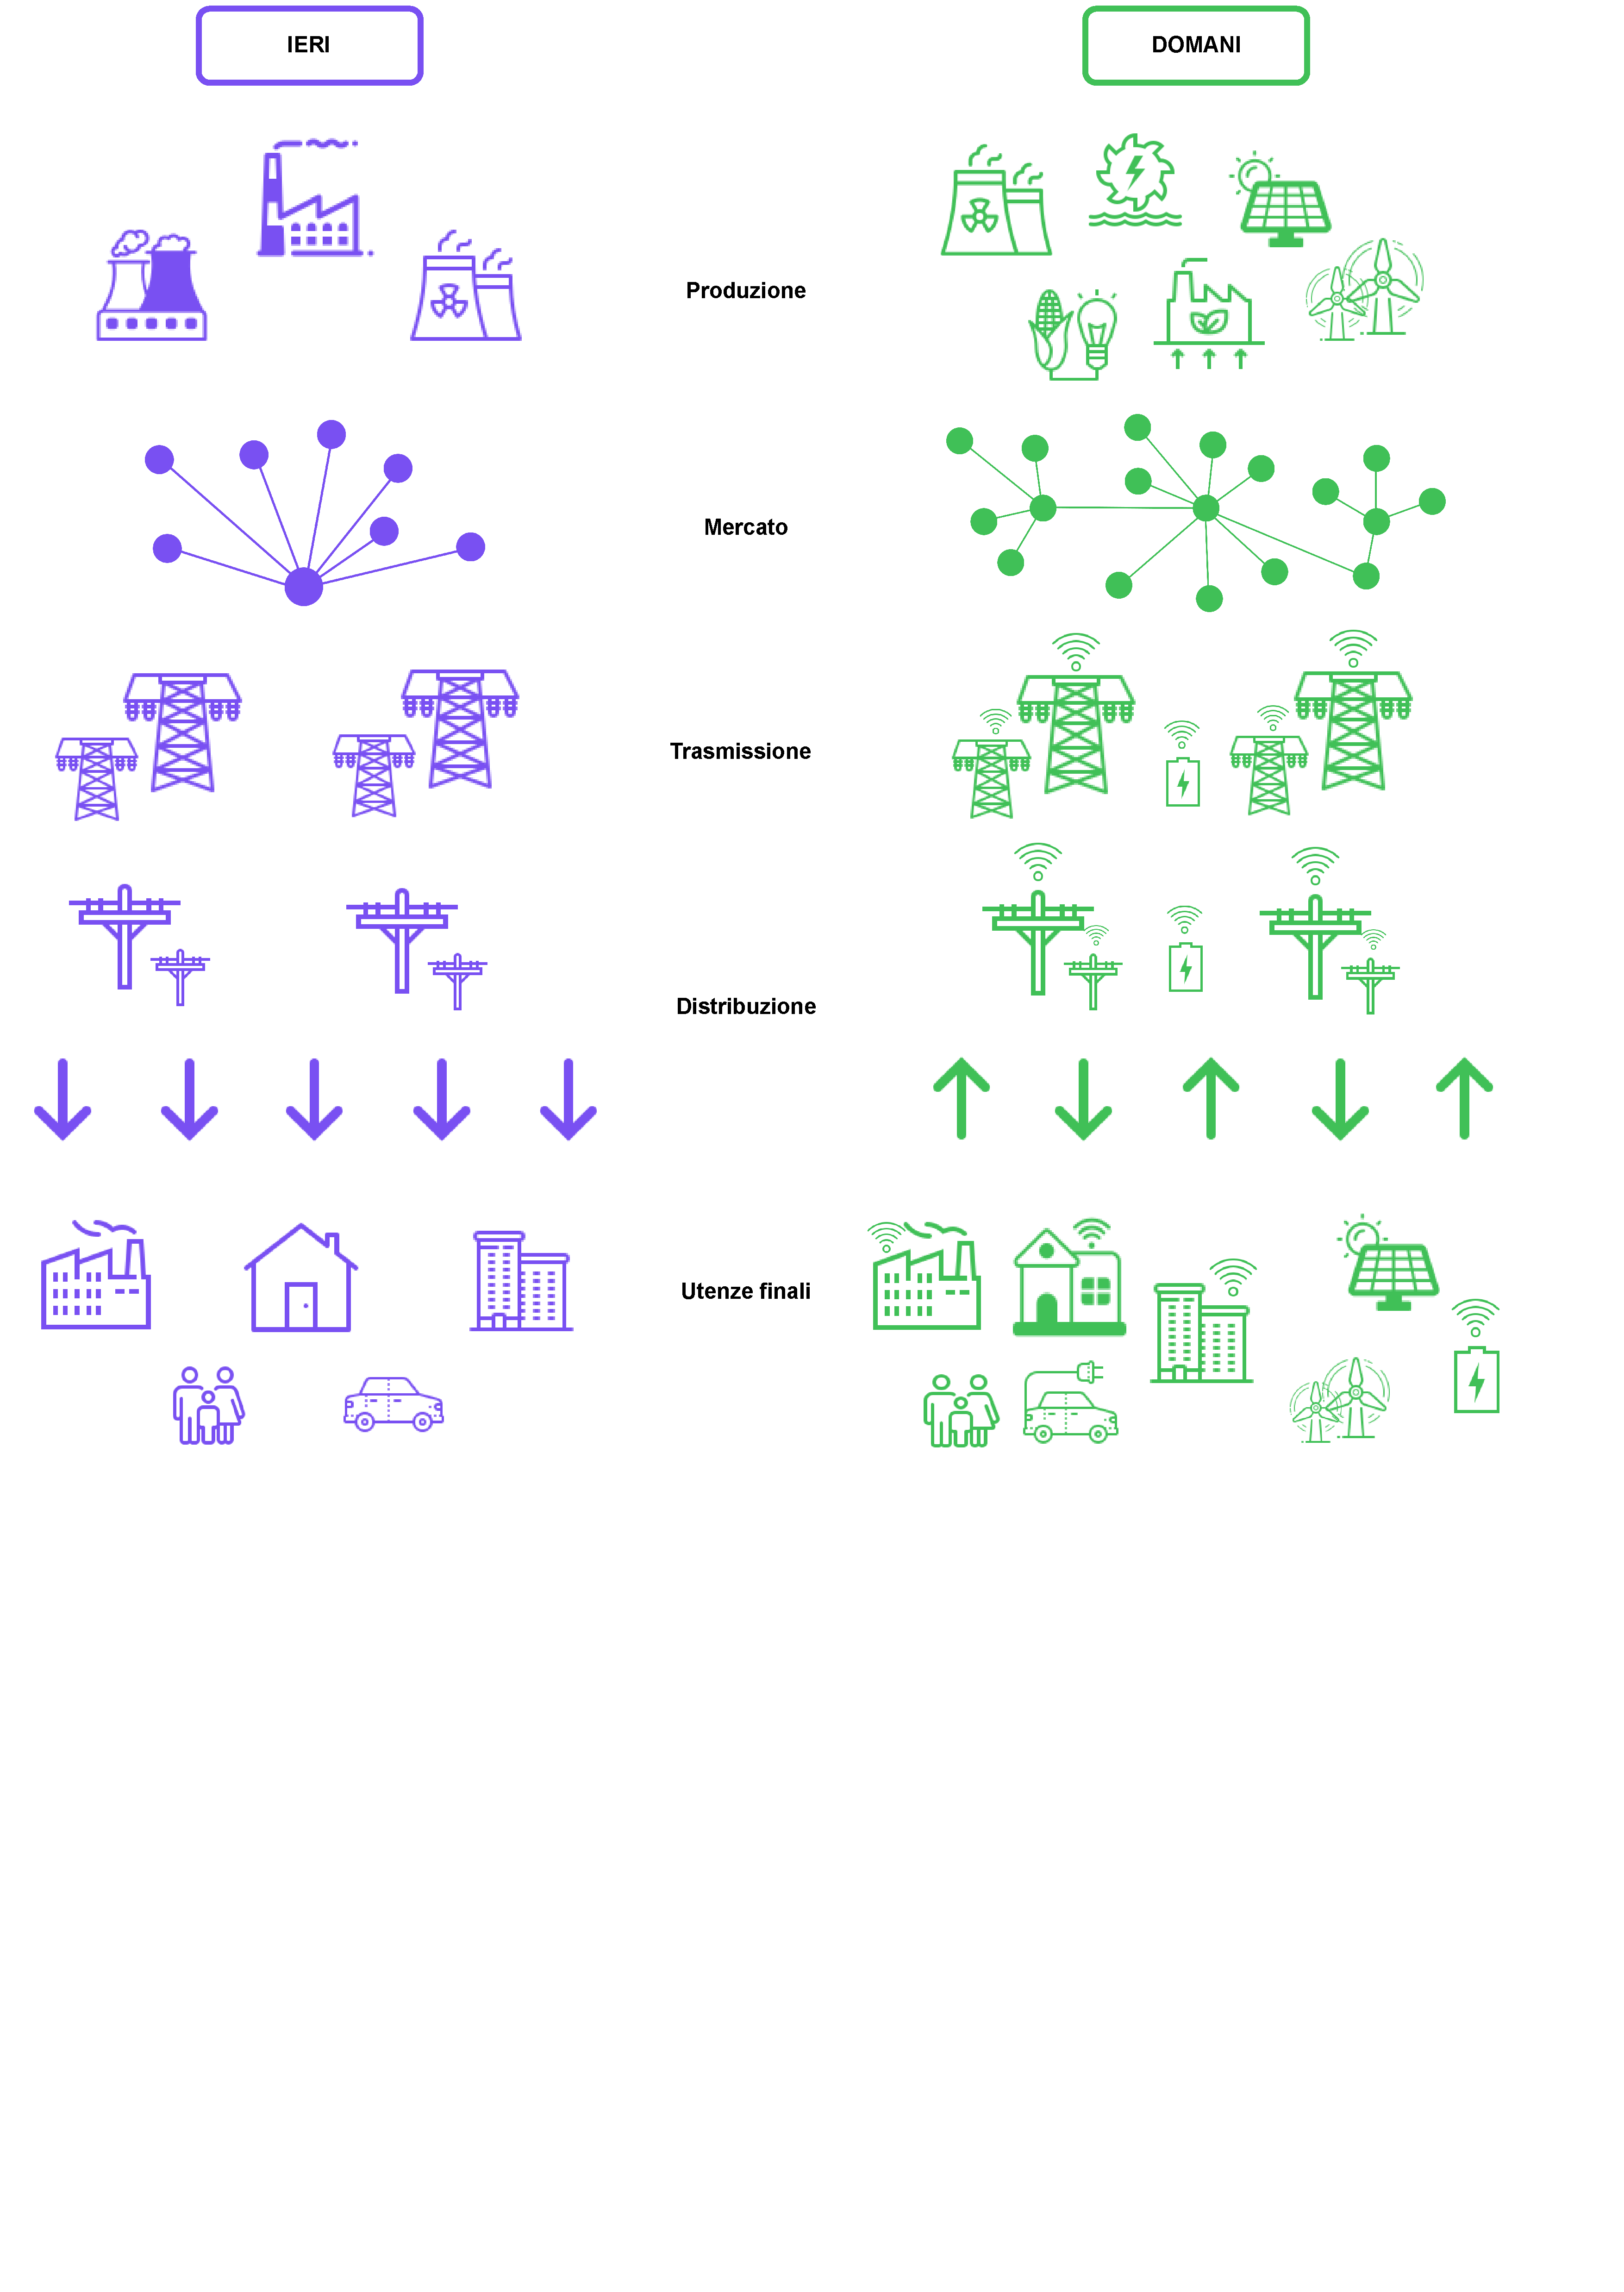
\includegraphics[trim= 0cm 31cm 1cm 0cm, clip, width=0.8\linewidth]{img/SM-no-bg.drawio.pdf}
%     \caption{Confronto rete tradizionale e rete intelligente}
%     \label{fig:TraditionalGridVSSmartrGrid}
% \end{figure}

\begin{figure}[h!]
    \centering
    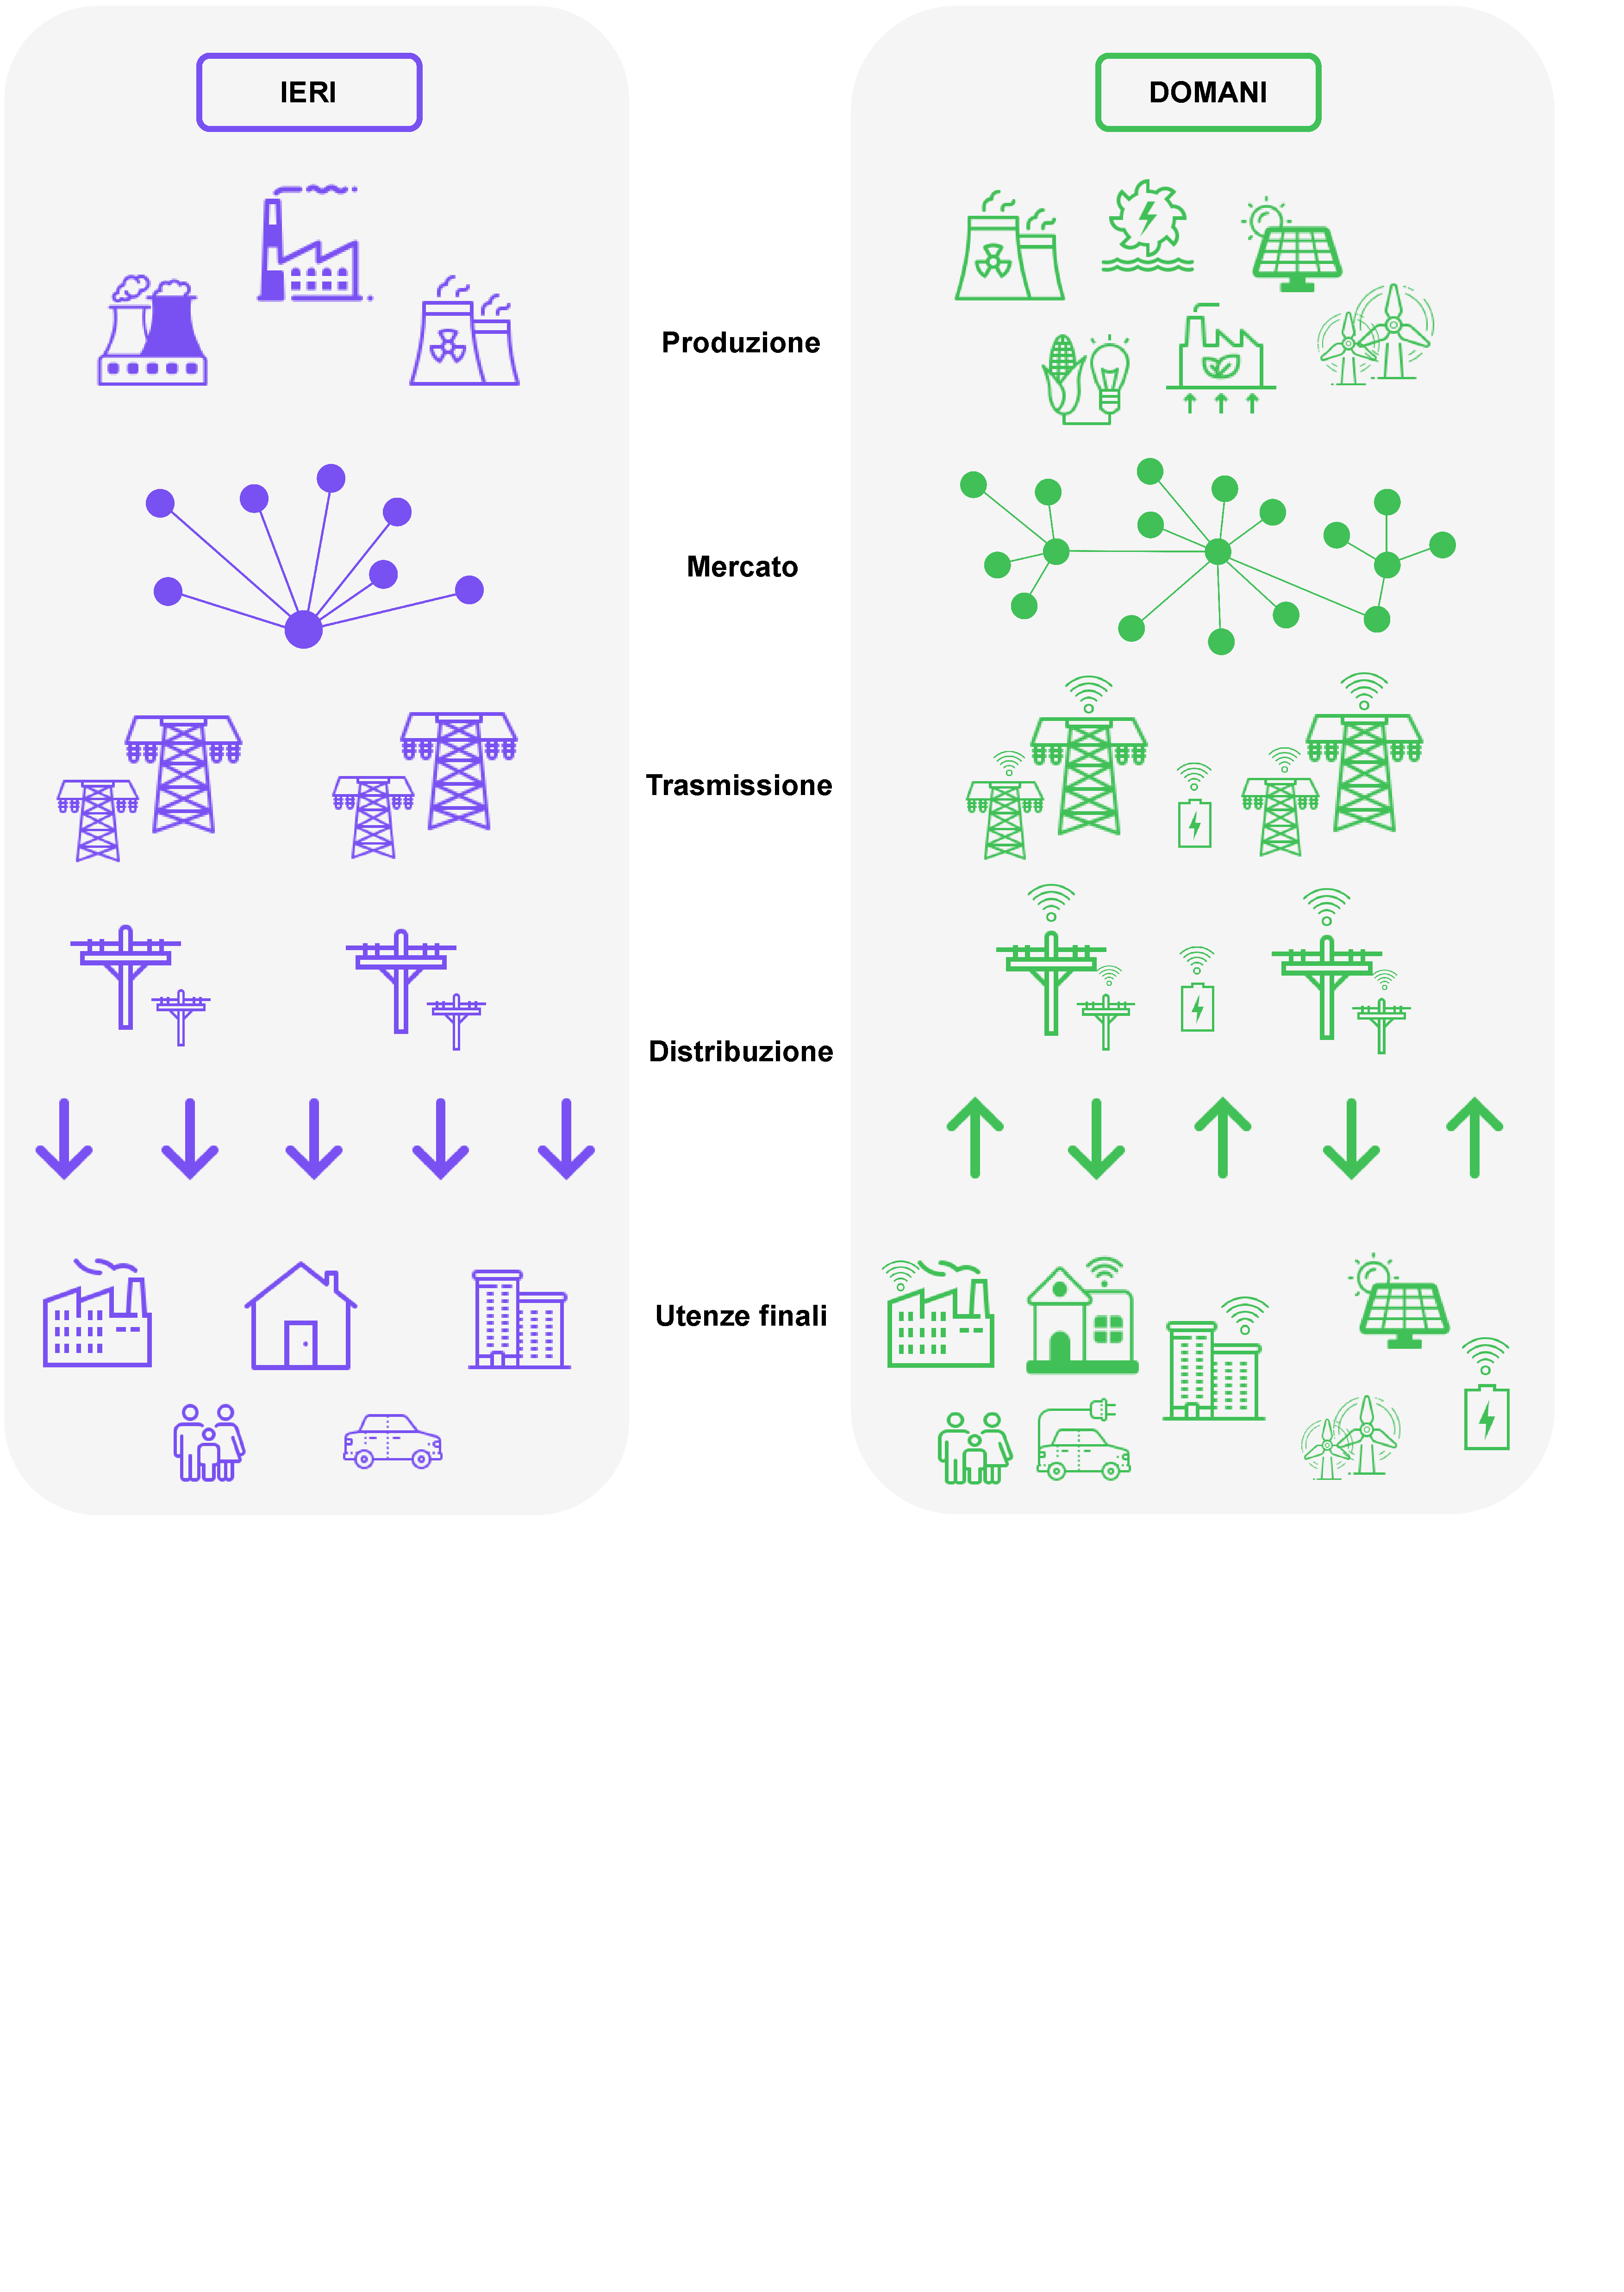
\includegraphics[trim= 0cm 28cm 0cm 0cm, clip, width=0.7\linewidth]{img/SM-gray-BG.drawio.pdf}
    \caption{Confronto rete tradizionale e rete intelligente}
    \label{fig:TraditionalGridVSSmartrGrid}
\end{figure}


% \begin{figure}[h!]
%     \centering
%     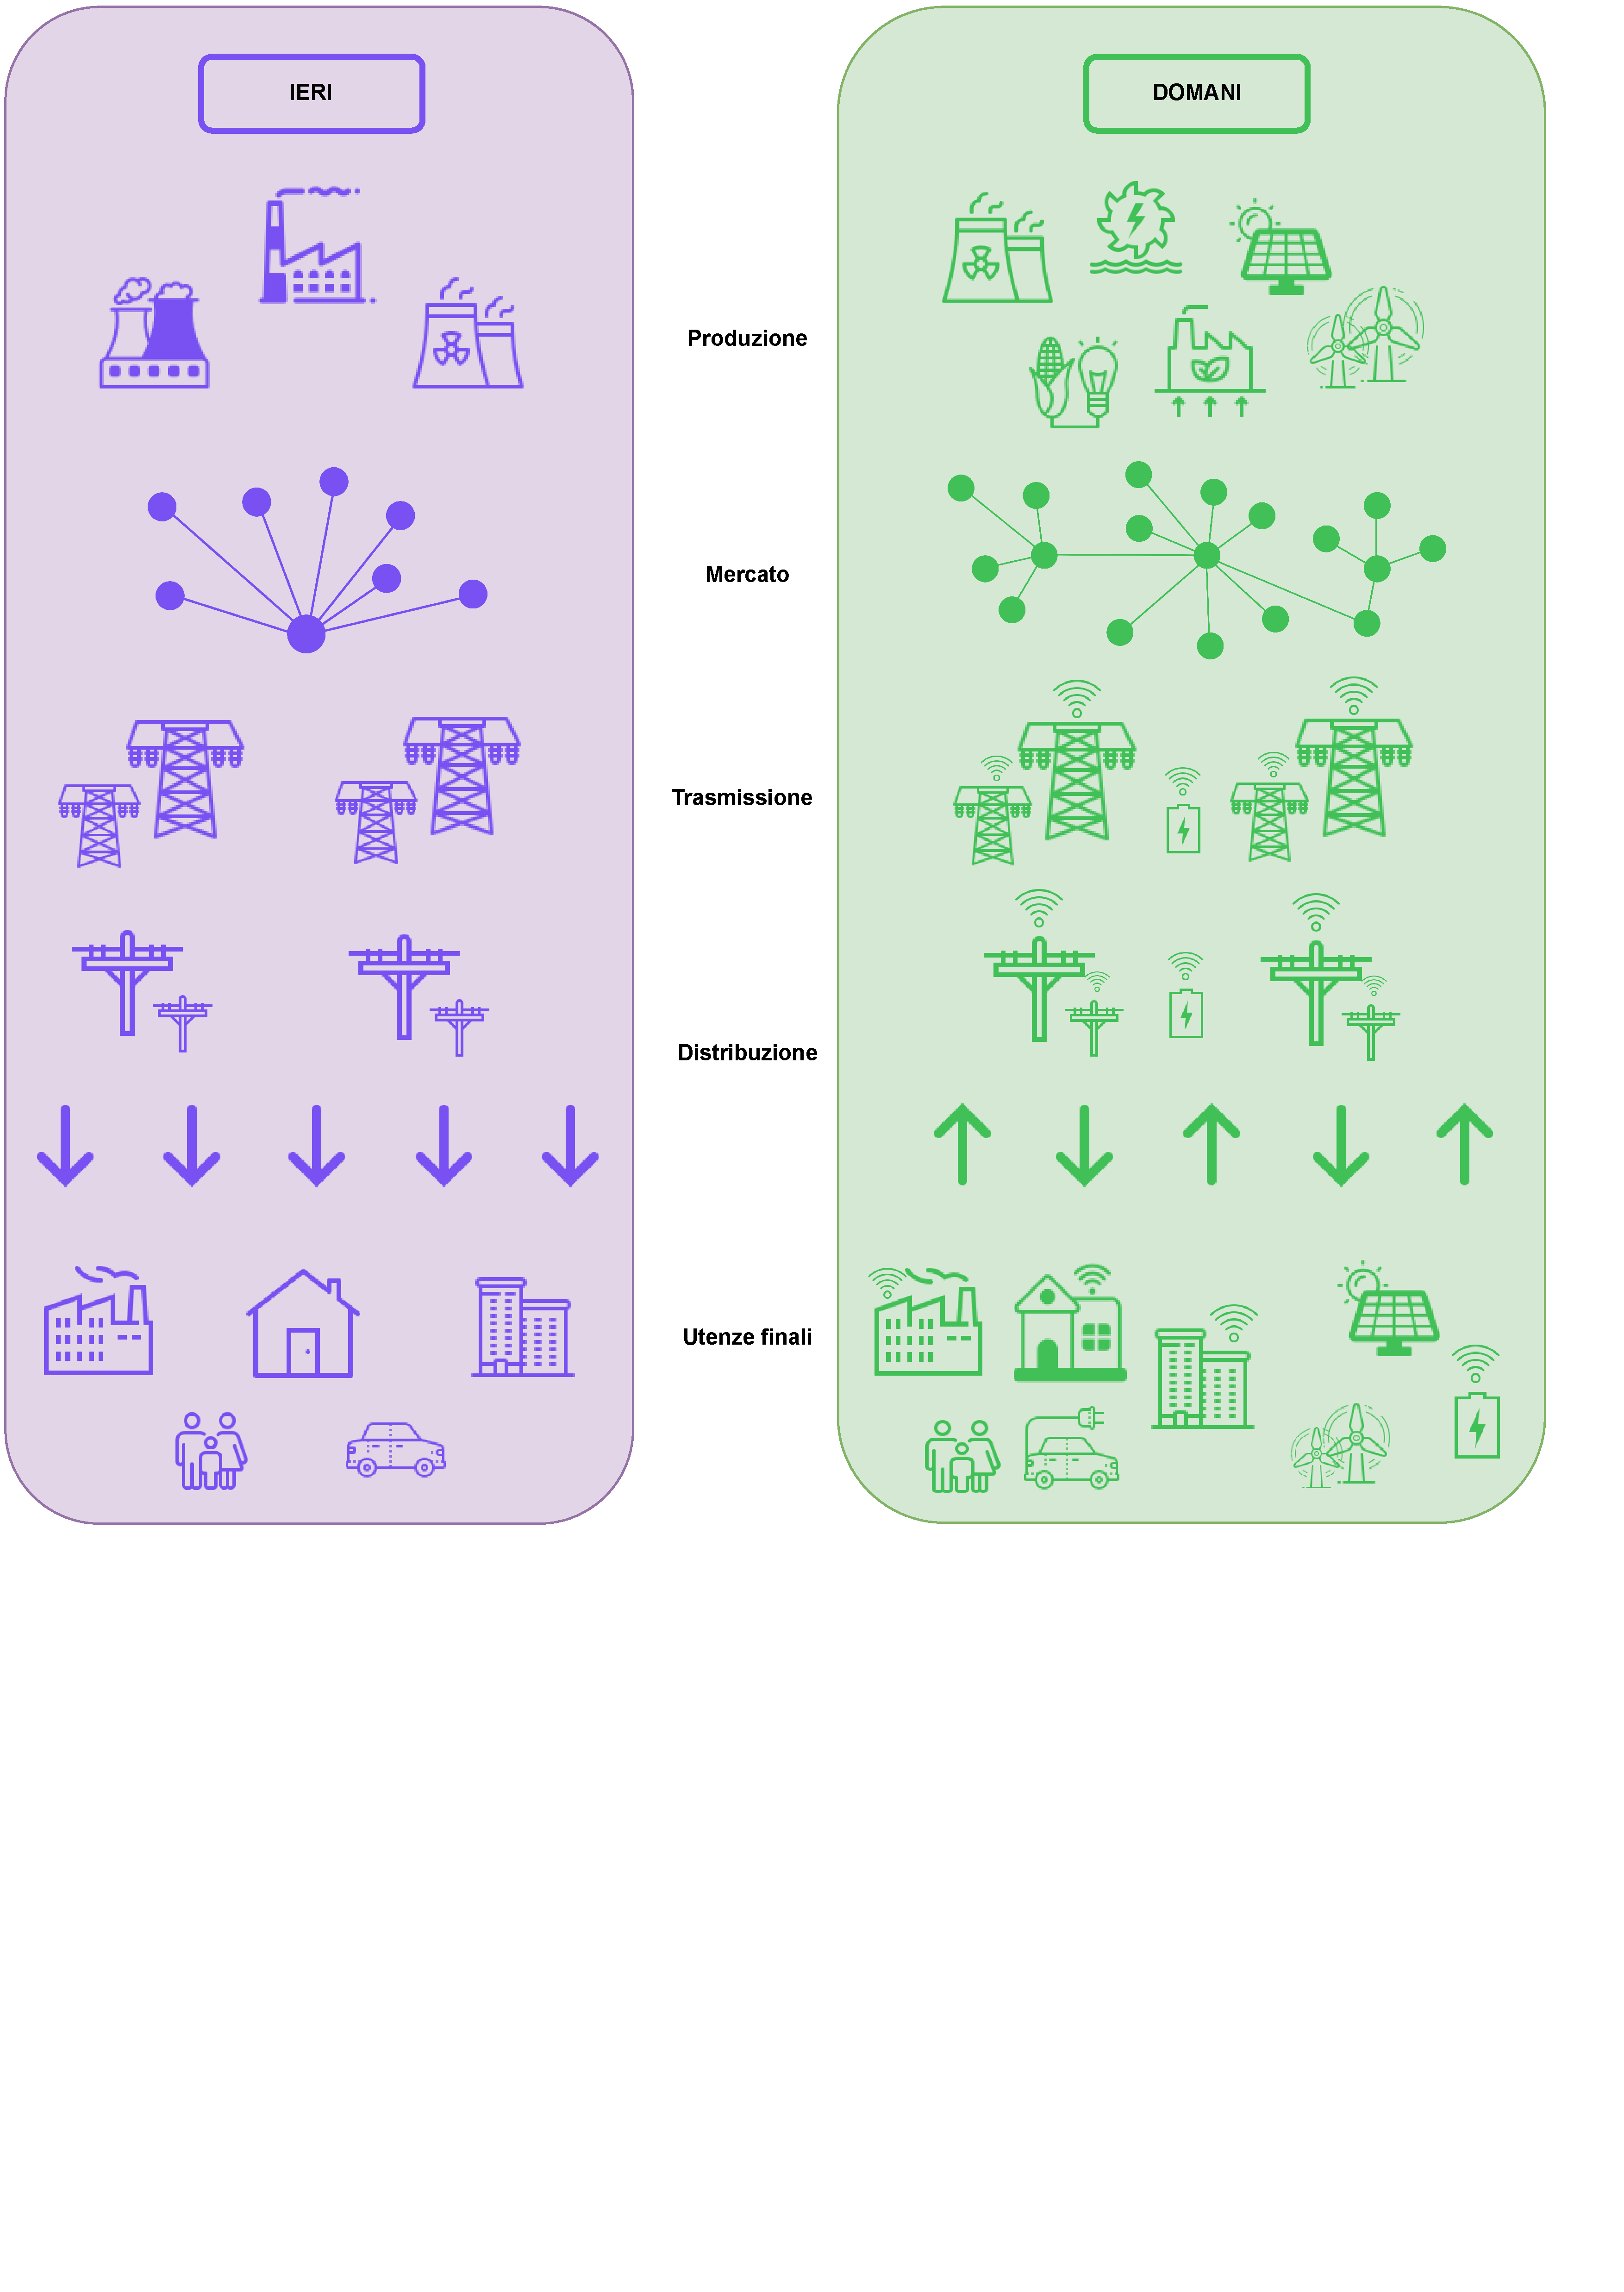
\includegraphics[trim= 0cm 28cm 1cm 0cm, clip, width=0.8\linewidth]{img/SM-colore-bg.drawio.pdf}
%     \caption{Confronto rete tradizionale e rete intelligente}
%     \label{fig:TraditionalGridVSSmartrGrid}
% \end{figure}


Come si può vedere nella Figura \ref{fig:TraditionalGridVSSmartrGrid} la Smart Grid si compone di 5 parti fondamentali: la Produzione, il Mercato\footnote{Non trattato in questa tesi}, la Trasmissione, la Distribuzione e infine le Utenze.

Nell'Allegato \ref{allegato:da-prod-alla-distrib} viene approfondita tutta la filiera  dell'energia, dal Produttore al Consumatore.

% \begin{center}
%     \textit{Produzione} - \textit{Trasmissione} - \textit{Distribuzione} - \textit{Utenze}
% \end{center}

%  ---------------------------- AGGEGATO -------------------------------------

% \newpage
% \subsection{Produzione dell'Energia: il Mix Energetico}

% \begin{figure}[t]
%     \centering
%     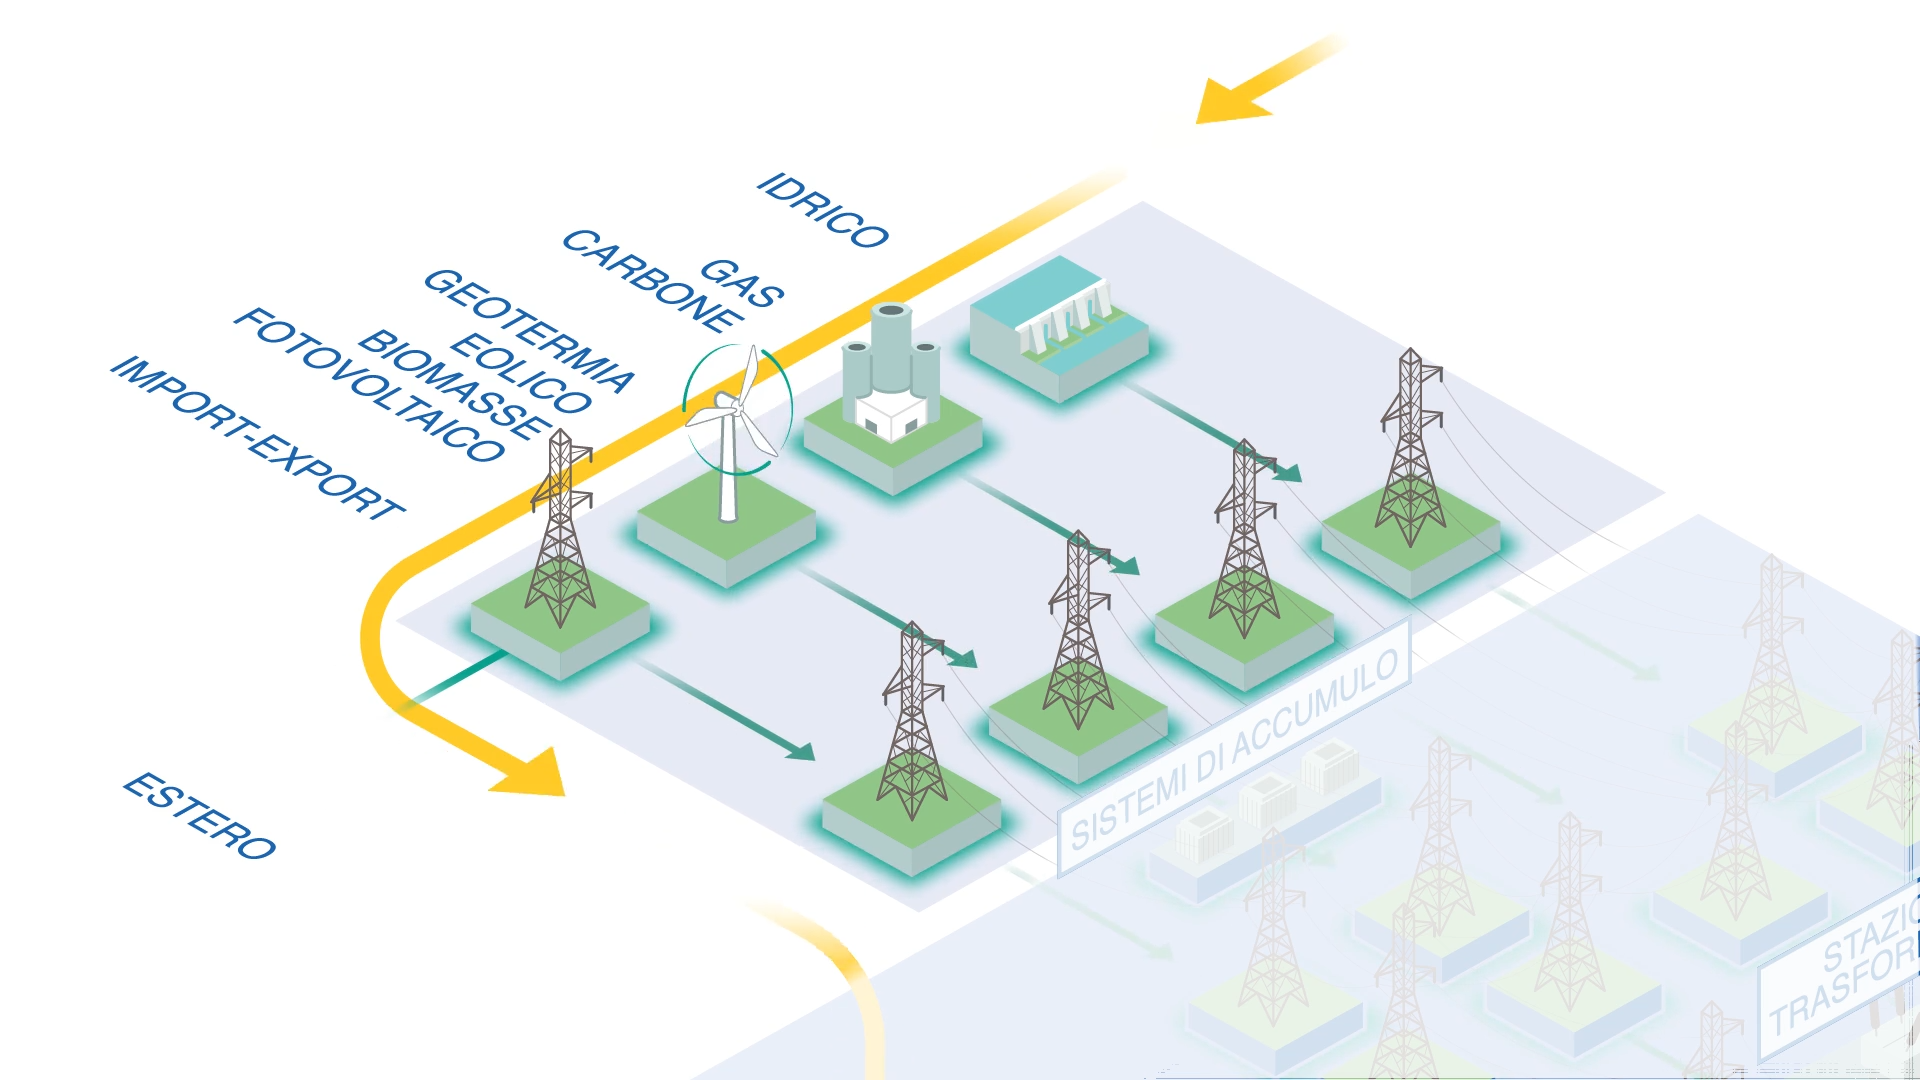
\includegraphics[width=0.45\linewidth]{img/Terna-Produzione.png}
%     \caption{Fonte immagine: Terna - Produzione}
% \end{figure}

% % La produzione di elettricità, sia nel sistema tradizionale sia con l'utilizzo delle Smart Grid, avviene attraverso un mix energetico di Fonti Energetiche non Rinnovabili (\textbf{non FER}) e Fonti Energetiche Rinnovabili (\textbf{FER}).

% % nuovo
% La generazione di energia elettrica, sia nei sistemi tradizionali che nelle Smart Grid, si fonda su un \textbf{mix energetico} che bilancia Fonti Energetiche non Rinnovabili (non-FER) e Fonti Energetiche Rinnovabili (FER), Tabella \ref{tab:GSE-mix-nazionale-2023}. Questo equilibrio è un fattore chiave per la stabilità e la sostenibilità del sistema elettrico nazionale.
% % fine nuovo

% % Il mix energetico italiano sfrutta varie fonti tra cui le non FER, con circa il 54\%, e il restante 46\% proviene invece dalle fonti FER Tabella \ref{tab:GSE-mix-nazionale-2023}.

% \vspace{-0.4cm}
% \begin{table}[h!]
%     \renewcommand{\arraystretch}{1.4}
%     \centering
%     \begin{tabular}{lc}
%         % \multicolumn{2}{c}{\shortstack{}}\\
%          % \multicolumn{2}{c}{Fonti primarie utilizzate \%} \\
%          \hline
%          \textbf{Fonti primarie utilizzate}	& \textbf{\%} \\
%          \hline
%          Fonti rinnovabili & 46 \\
%          Gas naturale& 43 \\
%          Carbone& 5 \\
%          Altre fonti & 5 \\
%          Prodotti petroliferi& 1 \\
%          \hline
%     \end{tabular}
%     \caption{Composizione del mix iniziale nazionale immessa nel anno 2023 \cite{GSE}}
%     \label{tab:GSE-mix-nazionale-2023}
% \end{table}

% \vspace{-0.4cm}


% % \renewcommand{\arraystretch}{1.5}
% % \begin{longtable}[!h]{p{5cm}p{0.5cm}}

        
% %     \caption{Composizione del mix iniziale nazionale immessa nel anno 2023 \cite{GSE}}
% %     \label{tab:GSE-mix-nazionale-2023}\\
    
% %     \hline
% %     \textbf{Fonti primarie utilizzate}	& \textbf{\%} \\
% %     \hline
% %     \endfirsthead
    
% %     \hline
% %     \textbf{Fonti primarie utilizzate}	& \textbf{\%} \\
% %     \hline
% %     \endhead
    
% %          Fonti rinnovabili & 46 \\
% %          Gas naturale& 43 \\
% %          Carbone& 5 \\
% %          Altre fonti & 5 \\
% %          Prodotti petroliferi& 1 \\
    
% %     \hline
% % \end{longtable}



% % \footnote{Non Trade adjusted - ovvero questi dati non sono stati corretti per import/export  }


% % In particolare, come riportato nel "Rapporto Mensile sul Sistema Elettrico 2024" redatto da Terna \cite{TernaRapporto2024}, si mostra che l'assorbimento totale, la somma di produzione più importazioni di energia elettrica, nel periodo Gen-Dic 2024 è stata di $312\,TWh$, di cui FER \footnote{Produzione da FER = Idrico + Biomasse + Geotermico + Eolico + Fotovoltaico} $129\,TWh\,(49\,\%)$, non FER $132\,TWh\ (51\,\%)$ e importazioni $51\,TWh$ principalmente da Francia e Svizzera.

% % nuovo
% Analizzando il contesto italiano, i dati più recenti del "Rapporto Mensile sul Sistema Elettrico" di Terna per il periodo Gennaio-Dicembre 2024 \cite{TernaRapporto2024} offrono un quadro preciso della situazione. A fronte di un assorbimento totale di energia elettrica di $312\,TWh$, la produzione nazionale netta si è attestata a $261\,TWh$. La composizione di tale produzione evidenzia un contributo quasi paritetico tra fonti rinnovabili e non rinnovabili. In particolare, $132\,TWh\ (51\,\%)$ della produzione è derivato da fonti non-FER, mentre $129\,TWh\,(49\,\%)$ è stato generato da FER, a testimonianza del progresso della transizione energetica. Il fabbisogno è stato infine completato da un saldo netto di importazioni dall'estero per $51\,TWh$, principalmente da Francia e Svizzera.
% % fine nuovo



% \begin{figure}[h!]
%     \centering
%     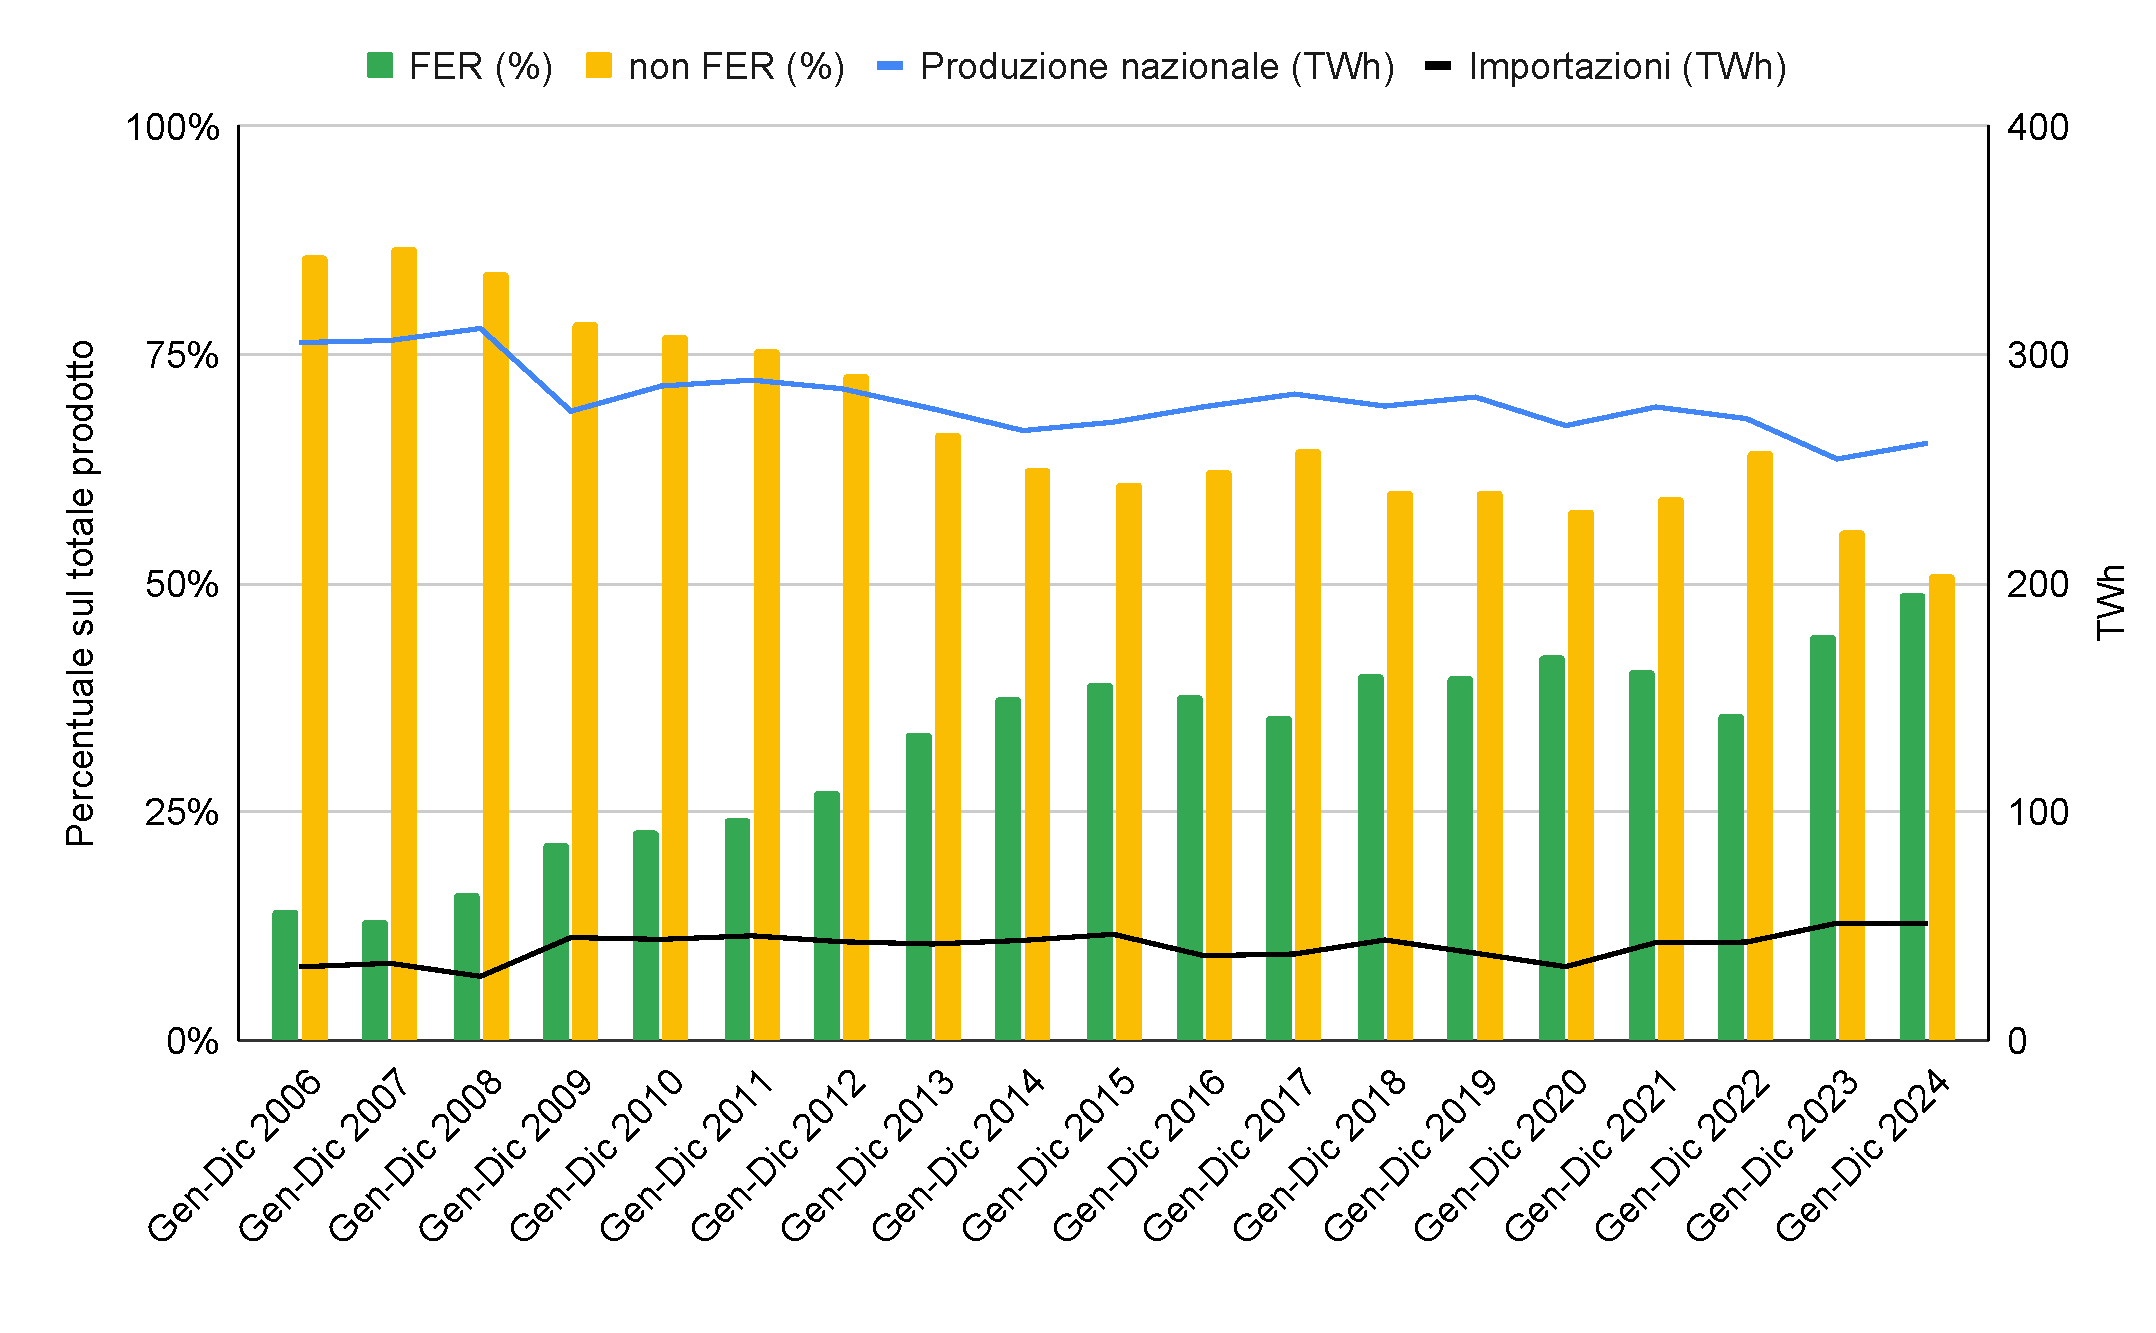
\includegraphics[trim= 0cm 1.5cm 0cm 0cm, clip, width=0.7\linewidth]{img/Terna-rapporto-annuale-2006-2024-v2.pdf}
%     \caption{Produzione nazionale annuale suddivisa tra FER e non FER \cite{terna-rapporto-mensile-sito}}
%     \label{graph:Terna-rapporto-annuale-2006-2024}
% \end{figure}

% % Si può vedere dal Grafico \ref{graph:Terna-rapporto-annuale-2006-2024} come dal 2006 al 2024 ci sia stato un incremento consistente della produzione di energia attraverso le fonti FER, arrivando quasi ad un break even nel 2024. In particolar modo, come si evince dal Grafico \ref{graph:Terna-FER-a-confronto-2006-2024}, questa crescita è stata possibile grazie all'installazione di pannelli fotovoltaici a partire dall'anno 2009 e il progressivo e costante aumento degli impianti eolici.


% % nuovo
% La crescente rilevanza delle fonti rinnovabili non è un fenomeno recente, ma il risultato di un trend consolidato. Come evidenziato nel Grafico \ref{graph:Terna-rapporto-annuale-2006-2024}, il periodo dal 2006 al 2024 ha visto un incremento costante e significativo della produzione da FER, fino a raggiungere quasi un punto di pareggio con le fonti convenzionali nell'ultimo anno di rilevazione. L'analisi disaggregata di questa crescita, Grafico \ref{graph:Terna-FER-a-confronto-2006-2024}, rivela che i principali motori di questa trasformazione sono stati l'espansione del settore fotovoltaico, a partire dal 2009, e lo sviluppo continuo e progressivo dell'energia eolica.
% % fine nuovo

% \begin{figure}[h!]
%     \centering
%     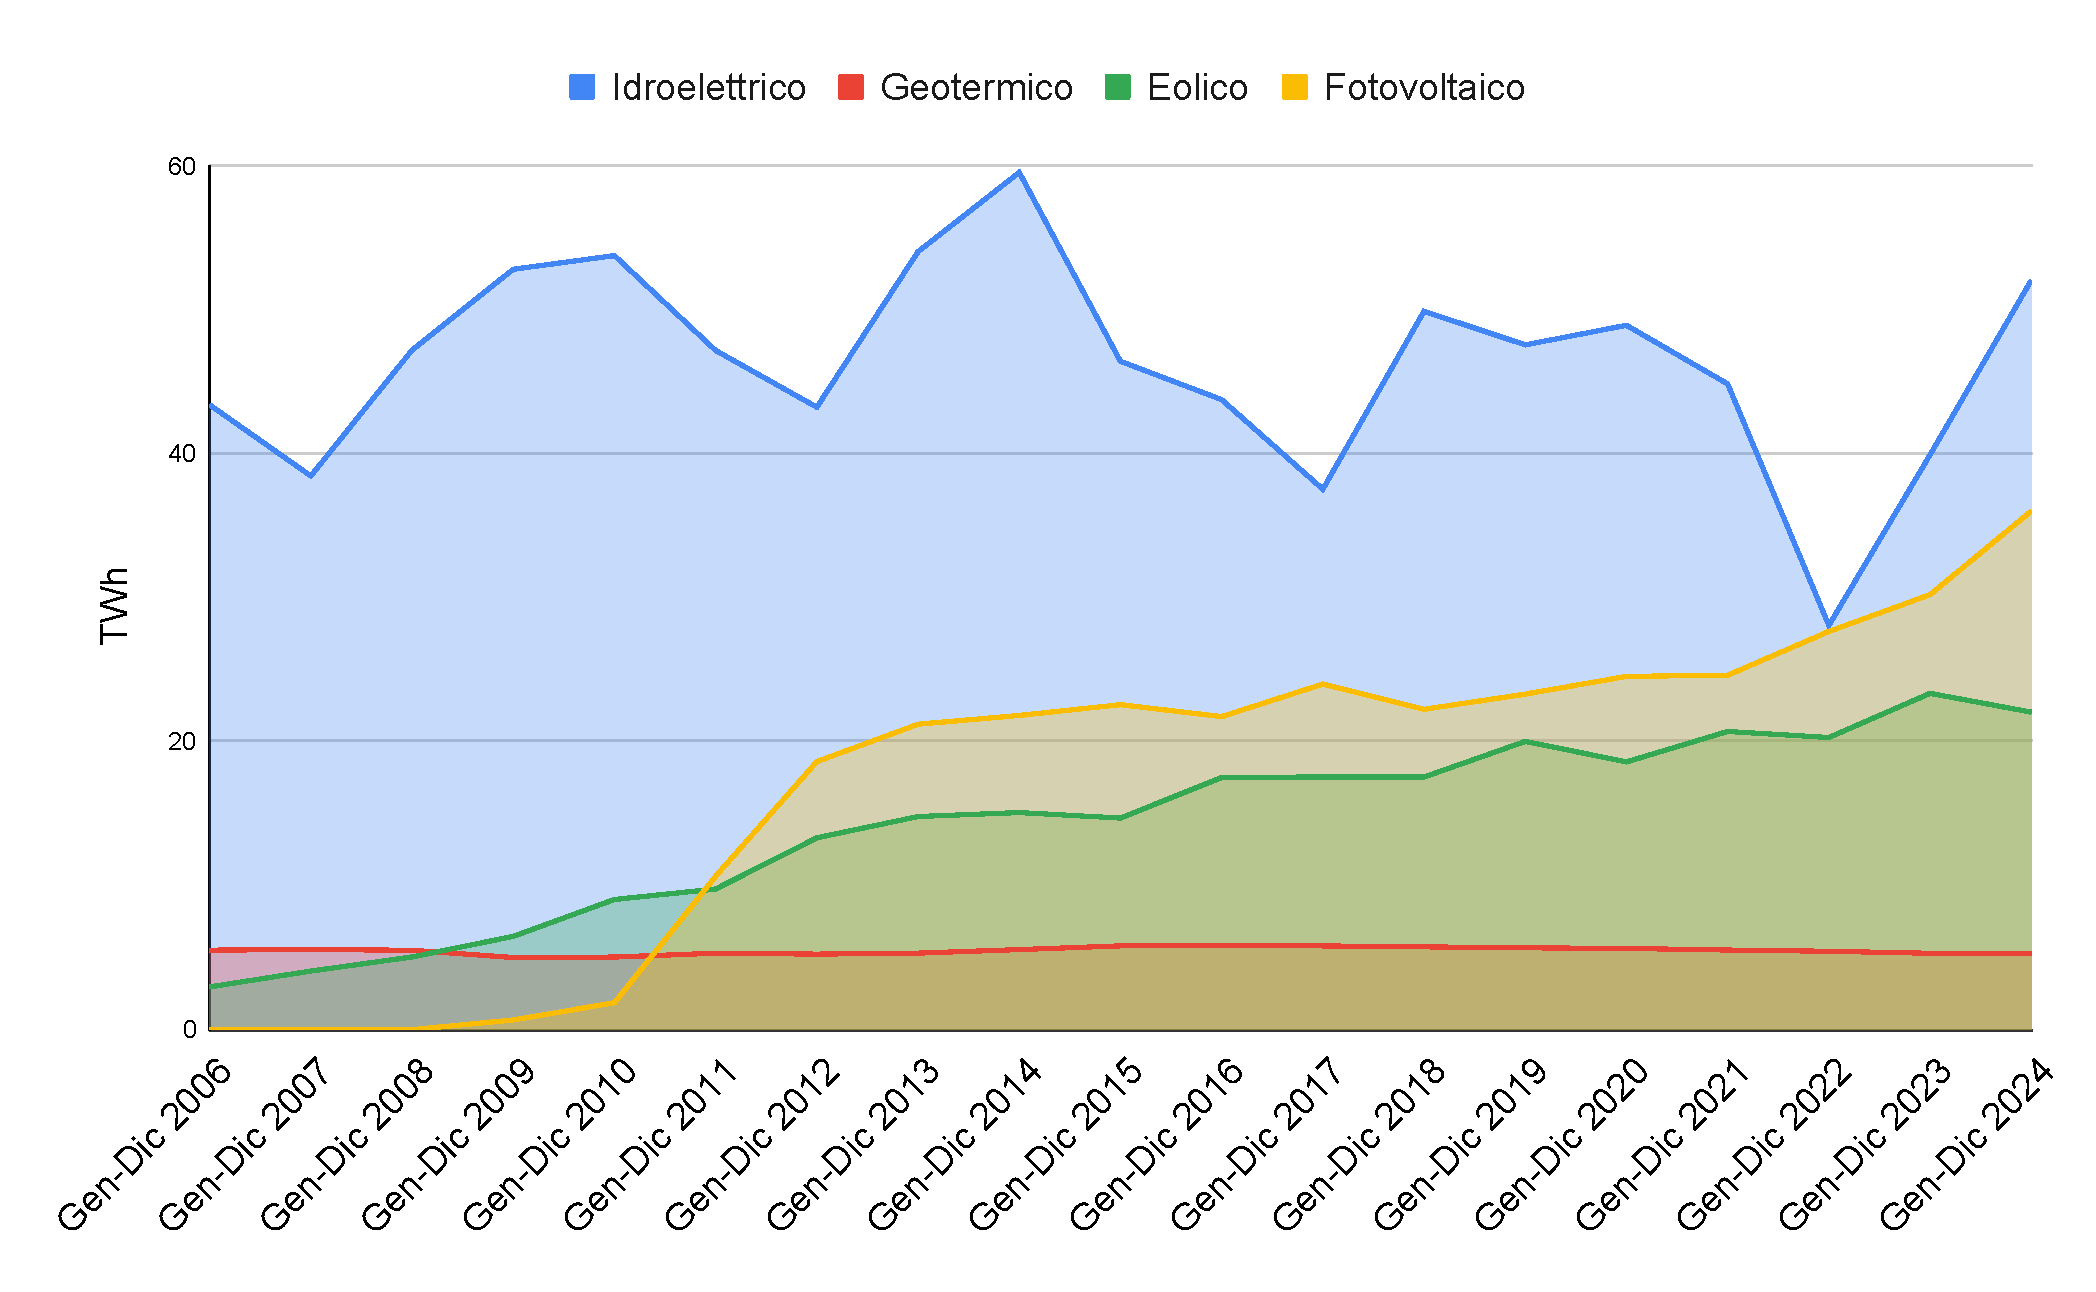
\includegraphics[trim= 0cm 1cm 0cm 1.05cm, clip, width=0.7\linewidth]{img/Terna-FER-a-confronto-2006-2024-v2.pdf}
%     \caption{Suddivisione delle principali FER in Italia \cite{terna-rapporto-mensile-sito}}
%     \label{graph:Terna-FER-a-confronto-2006-2024}
% \end{figure}


% \begin{figure}[b]
%     \centering
%     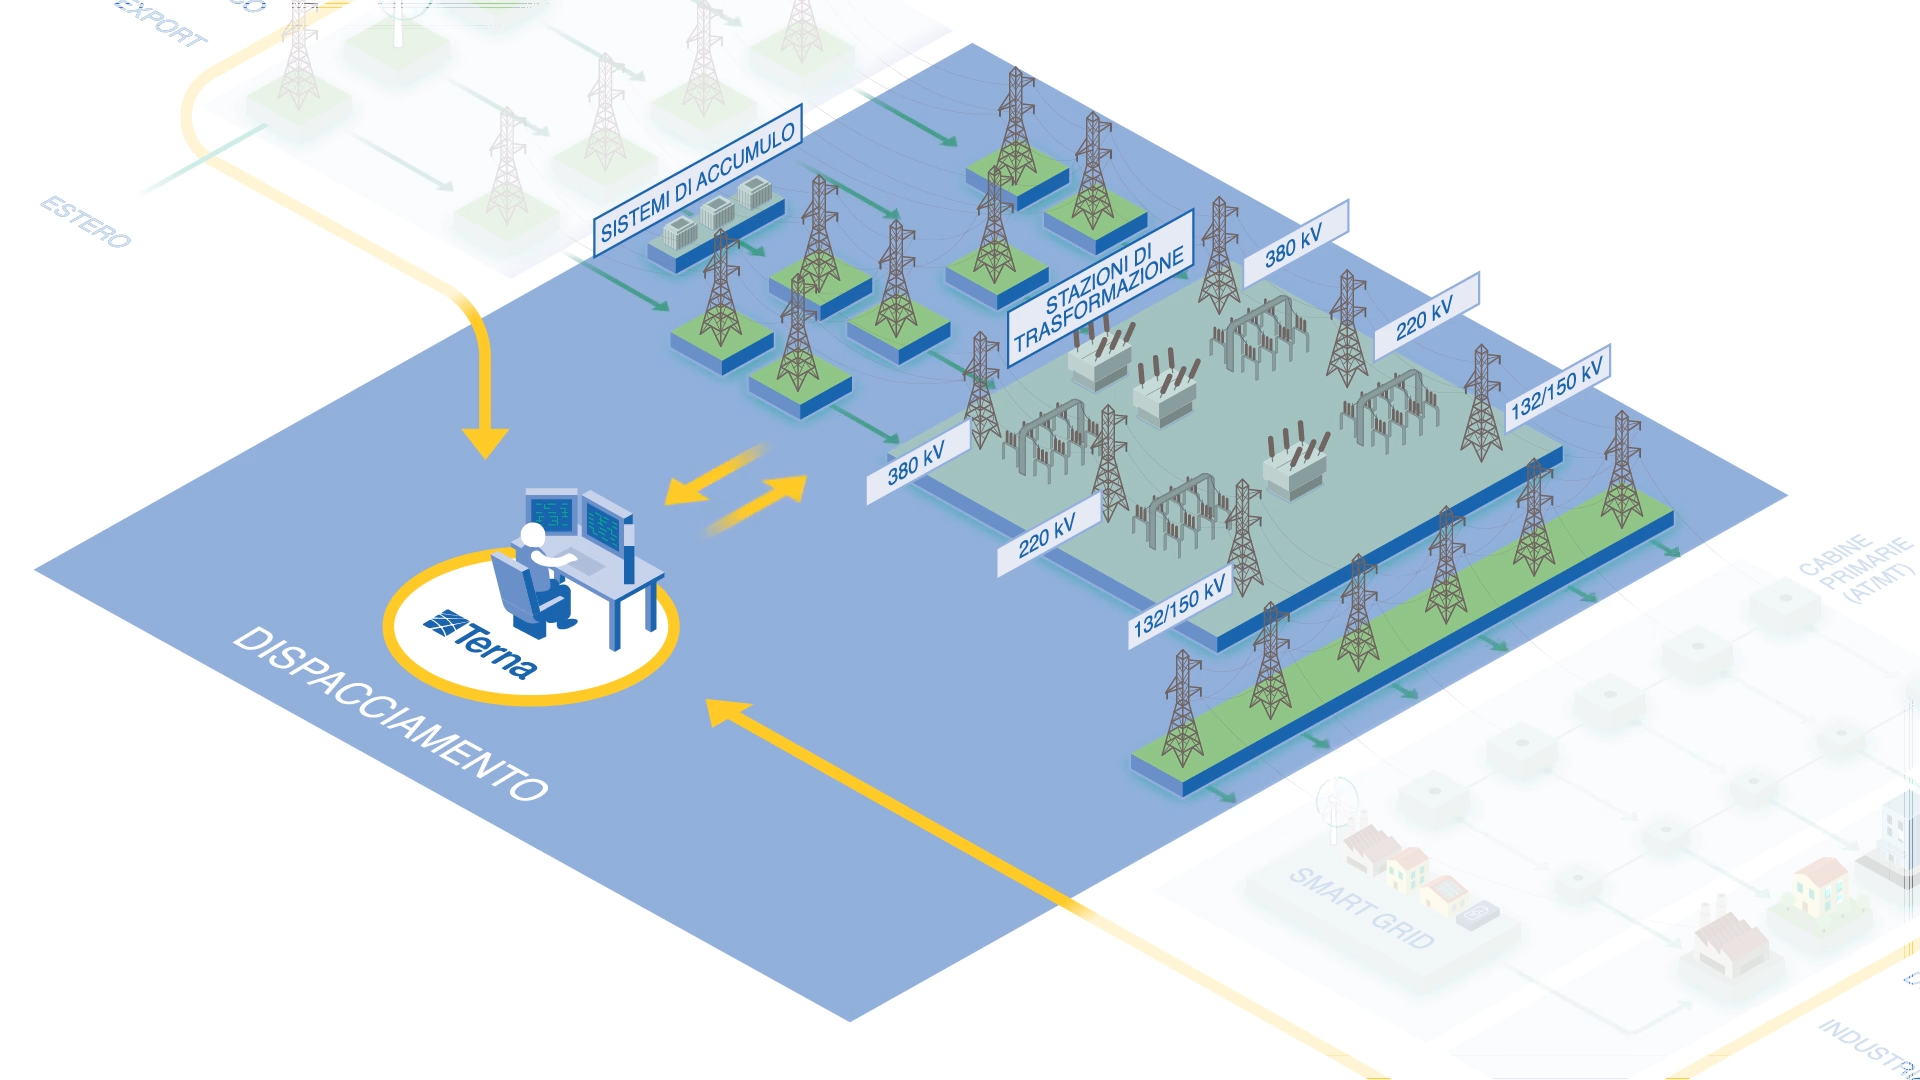
\includegraphics[width=0.5\linewidth]{img/Terna-Trasmissione.png}
%     \caption{Fonte immagine: Terna - Trasmissione}
% \end{figure}


% \subsection{La Trasmissione e il Dispacciamento dell'Energia}
% % La società italiana che, in un regime di monopolio naturale, si occupa della trasmissione e del dispacciamento è Terna. Questa modalità di governance è diffusa anche nel resto d'Europa, poiché è la configurazione ideale da mantenere per garantire una gestione, un mantenimento e uno sviluppo costante su tutta la Rete Elettrica Nazionale (RTN).

% La fase di trasmissione costituisce il sistema nervoso della rete elettrica, incaricata di trasportare l'energia su lunghe distanze, dalle centrali di produzione alle reti di distribuzione. In Italia, questa infrastruttura strategica, nota come Rete di Trasmissione Nazionale (RTN), è gestita in regime di monopolio naturale da \textbf{Terna}, che opera in qualità di \textit{Transmission System Operator} (TSO). Tale modello di governance, diffuso in gran parte d'Europa, è considerato ottimale per garantire l'efficienza, la sicurezza e lo sviluppo coordinato dell'intera infrastruttura elettrica nazionale.

% % La trasmissione è un punto cruciale del dispacciamento dell'energia elettrica che comprende: 

% % \begin{itemize}
% %     \item il monitoraggio dei flussi energetici deviando l'energia nelle zone con più alto assorbimento
% %     \item le procedure operative per il controllo coordinato di tutti i componenti sistemici
% %     \item la programmazione di riparazioni, l'allaccio di nuove linee e l'indisponibilità di pezzi della rete
% %     \item la previsione del fabbisogno energetico nazionale ora per ora
% % \end{itemize}


% \subsubsection{Funzioni del TSO: Il Dispacciamento}

% Il ruolo di Terna non si limita alla manutenzione fisica della rete, ma include la complessa attività di dispacciamento: la gestione e il controllo in tempo reale dei flussi energetici per assicurare costantemente l'equilibrio tra energia prodotta e consumata. 

% Le principali responsabilità del dispacciamento includono:

% \begin{itemize}
%     \item il \textbf{monitoraggio} continuo dei flussi di potenza e la loro deviazione per soddisfare i picchi di assorbimento regionali;
%     \item l'attuazione di \textbf{procedure operative} per il controllo coordinato di tutti gli elementi del sistema (centrali, linee, stazioni);
%     \item la \textbf{pianificazione} delle manutenzioni, dell'allacciamento di nuove linee e della gestione delle indisponibilità programmate o accidentali di porzioni della rete;
%     \item la \textbf{previsione} del fabbisogno energetico nazionale con un dettaglio orario, fondamentale per la programmazione della produzione.
% \end{itemize}


% % Tutto questo tenendo sempre in considerazione che la sinusoide di rete, dalla produzione all'utente finale viene impiegata una corrente alternata, in tutta Italia - ed Europa - deve, in qualsiasi istante, avere una frequenza nominale ($f_n$) di $50\,Hz$ con possibile funzionamento senza limiti di tempo (condizioni normali) da $47,5\,Hz$ a $51,5\,Hz$, e una tensione nominale di rete, indicata con $U_n$, di $230\,V$ per le forniture monofase e $400\,V$ per le forniture trifase, con tolleranze di $\pm 10\,\%$ ovvero da $207\,V$ a $253\,V$ e da $360\,V$ a $440\,V$. \cite{Fase-di-rete-terna} \cite{CEI0-21}

% % La sinusoide di rete utilizza corrente alternata dalla produzione all'utente finale. In tutta Italia ed Europa, questa deve mantenere parametri specifici in qualsiasi istante.


% % La frequenza nominale ($f_n$) è di $50\,Hz$ . In condizioni normali, può funzionare senza limiti di tempo tra $47,5\,Hz$ e $51,5\,Hz$.\cite{Fase-di-rete-terna} 


% % La tensione nominale di rete ($U_n$) è di $230\,V$ per le forniture monofase e $400\,V$ per le forniture trifase, con tolleranze ammesse di $\pm 10\,\%$ \cite{CEI0-21}, quindi:


% % \begin{center}
% %     Monofase: $207\,V$ a $253\,V$ e Trifase: $360\,V$ a $440\,V$
% % \end{center}

% % \begin{itemize}
% %     \item[] Monofase: $207\,V$ a $253\,V$
% %     \item[] Trifase: $360\,V$ a $440\,V$
% % \end{itemize}




% % Un, Vn soo differenti!


% % Principalmente al livello di trasmissione si lavora ad Alta ed Altissima tensione, rispettivamente da $35\,kV < U \leq 220\,kV$ e oltre i $220\,kV$\cite{alta-tensione-parametri}. L'utilizzo di linee ad elevato potenziale è dettata dalla necessità di limitare la corrente su di esse e dunque ridurre drasticamente le perdite di energia per effetto Joule.



% \subsubsection{Parametri Tecnici della Rete di Trasmissione}

% Per garantire la stabilità e la qualità della fornitura, l'energia elettrica in corrente alternata deve rispettare parametri tecnici rigorosi in ogni punto della rete europea. I due principali indicatori sono la frequenza e la tensione.


% \begin{itemize}
%     \item \textbf{Frequenza}: La frequenza nominale ($f_n$) del sistema è fissata a $50\,Hz$. Deviazioni da questo valore indicano uno squilibrio tra produzione e consumo. In condizioni operative normali, la rete è progettata per funzionare a tempo indeterminato entro un intervallo di tolleranza compreso tra $47,5\,Hz$ e $51,5\,Hz$, con limiti eccezionali di breve durata fuori dalle precedenti soglie \cite{Fase-di-rete-terna} \cite{EN-50160}.
%     \item \textbf{Tensione}: A livello di utenza finale, la tensione nominale ($U_n$) è di $230\,V$ per le forniture monofase e $400\,V$ per quelle trifase, con una tolleranza ammessa di $\pm 10\,\%$\footnote{Monofase: da $207\,V$ a $253\,V$ e Trifase: da $360\,V$ a $440\,V$} \cite{CEI0-21}. Tuttavia, per minimizzare le perdite di energia per effetto Joule ($P = R \cdot I^2$) durante il trasporto su lunghe distanze, la trasmissione avviene a livelli di tensione molto più elevati. 
%     La RTN, infatti, opera prevalentemente in Alta Tensione (AT), tra $35\,kV$ e $220\,kV$, e in Altissima Tensione (AAT), oltre i $220\,kV$\cite{alta-tensione-parametri}.
% \end{itemize}



% \begin{figure}[b]
%     \centering
%     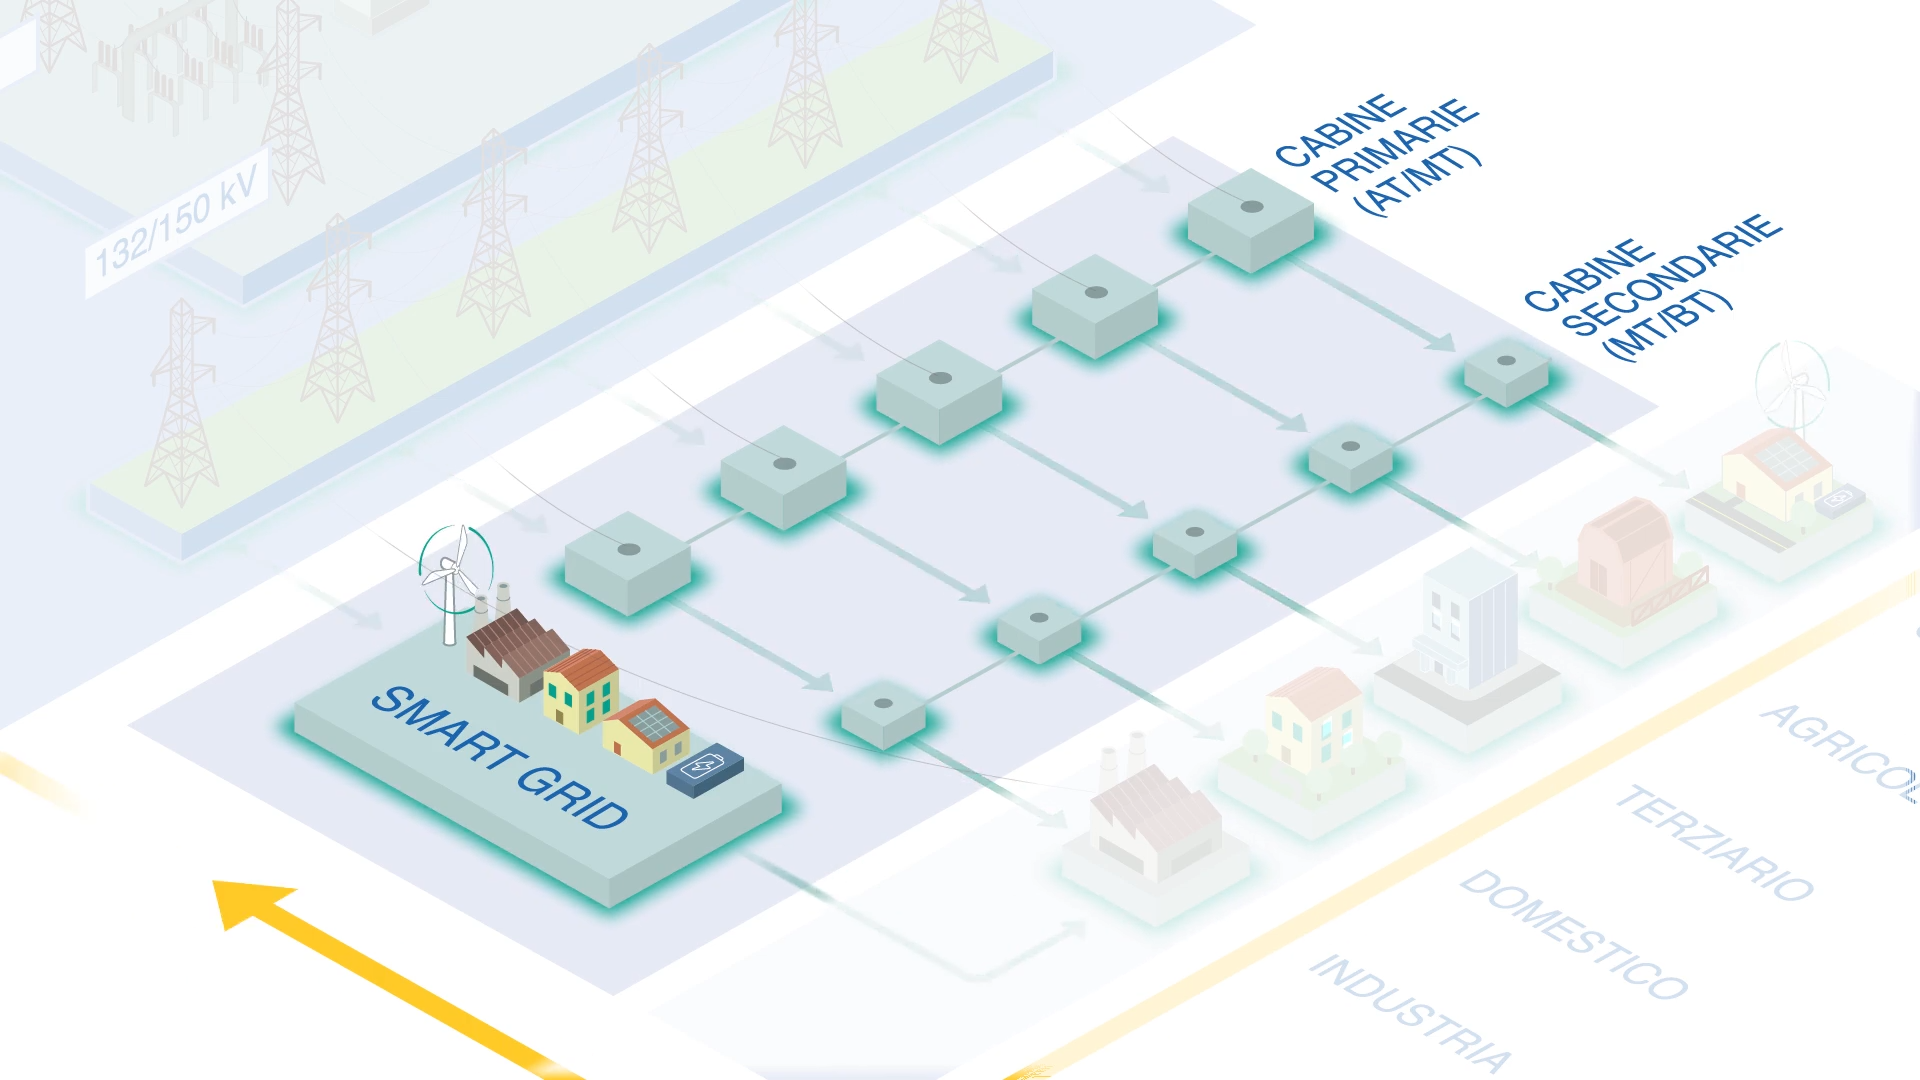
\includegraphics[width=0.5\linewidth]{img/Terna-Distribuzione.png}
%     \caption{Fonte immagine: Terna - Distribuzione}
% \end{figure}

% \subsection{La Distribuzione dell'Energia}

% % In Italia, se la trasmissione dell'energia elettrica è affidata a Terna tramite concessione statale, la distribuzione è invece gestita da diversi operatori attivi prevalentemente su base territoriale.

% La fase di distribuzione rappresenta il segmento finale della filiera elettrica, con il compito di prelevare l'energia dalla Rete di Trasmissione Nazionale (RTN) e consegnarla capillarmente agli utenti finali. A differenza della trasmissione, gestita da un singolo operatore nazionale, Terna, il servizio di distribuzione in Italia è frammentato e liberalizzato, operato su base territoriale da diversi \textit{Distribution System Operator} (DSO).

% % Attualmente sul territorio nazionale sono $114$ le aziende \cite{arera-distributori} che operano nel settore della distribuzione dell'energia elettrica

% Attualmente, sul territorio nazionale operano circa 114 aziende di distribuzione \cite{arera-distributori}. Sebbene il numero sia elevato, il mercato è fortemente concentrato. I principali DSO, che servono collettivamente la quasi totalità della popolazione italiana, sono elencati in Tabella \ref{tab:dso_italia}, la quale riporta per ciascuno il gruppo di appartenenza, il numero di utenti e l'area geografica di competenza. Tra questi, spicca E-Distribuzione, società del gruppo Enel, che da sola gestisce oltre 31 milioni di utenze \cite{Clienti-sertivi-distribuzione}.

% % I principali Distribution System Operator (DSO), che servono assieme la quasi totalità dei cittadini dell'intero territorio nazionale sono:

% % \begin{itemize}
    
% %     \item E-Distribuzione: società del Gruppo Enel con ben 31.1 milioni di utenti serviti  su tutto il territorio \cite{Clienti-sertivi-distribuzione}

% %     \item Areti: società del Gruppo Acea con 2,8 milioni di utenti operante nei territori di Roma e Formello \cite{Clienti-sertivi-areti}

% %     \item Unareti: società del Gruppo A2A con 1,2 milioni di utenti che gestisce i territori di Brescia, Milano e Bergamo \cite{Clienti-sertivi-uniareti}

% %     \item Ireti: società del Gruppo Iren con  700 mila utenti serviti nei territori di Parma, Torino e Vercelli \cite{Clienti-sertivi-ireti}

% %     \item Set Distribuzione: società del Gruppo Dolomiti Energia che serve il territorio della provincia autonoma di Trento con 330 mila utenze servite \cite{Clienti-sertivi-SetDistribuzione}

% %     \item V-reti: società del Gruppo AGSM AIM nata dall'integrazione tra Servizi a Rete (SAR) e Megareti. Sono 279 mila le utenze servite nel territorio di Verona e Vicenza  \cite{Clienti-sertivi-v-reti}

% %     \item InRete: società del Gruppo Hera distribuisce l'energia a oltre 264 mila utenti in Emilia-Romagna e in Toscana  \cite{Clienti-sertivi-edyna}

% %     \item Edyna: società del Gruppo Alperia, nata nel 2016 dalla fusione di Azienda EnergeticaReti e SELNET, distribuisce l'energia nel territorio altoatesino servendo 240 mila utenti.\cite{Clienti-sertivi-edyna}
        
% % \end{itemize}


% \begin{table}[h!]
% \renewcommand{\arraystretch}{1.5}
%     \centering
%     \begin{tabular}{ccclc}
%         % \hline
%         \hline
%         \textbf{DSO} & \textbf{Gruppo di} & \textbf{Utenti Serviti} & \textbf{Principali} & \textbf{Fonti} \\
%          & \textbf{Appartenenza} & \textbf{in mln.} & \textbf{aree geografiche} & \\
%         \hline
%         E-Distribuzione & Enel & 31,1 & Tutto il territorio nazionale & \cite{Clienti-sertivi-distribuzione} \\
%         % \hline
%         Areti & Acea & 2,8 & Roma e Formello & \cite{Clienti-sertivi-areti} \\
%         % \hline
%         Unareti & A2A & 1,2 & Brescia, Milano e Bergamo & \cite{Clienti-sertivi-uniareti} \\
%         % \hline
%         Ireti & Iren & 0,7 & Parma, Torino e Vercelli & \cite{Clienti-sertivi-ireti} \\
%         % \hline
%         Set Distribuzione & Dolomiti Energia & 0,3 & Provincia autonoma di Trento & \cite{Clienti-sertivi-SetDistribuzione} \\
%         % \hline
%         V-reti & AGSM AIM & 0,3 & Verona e Vicenza & \cite{Clienti-sertivi-v-reti} \\
%         % \hline
%         InRete & Hera & 0,3 & Emilia-Romagna e Toscana & \cite{Clienti-sertivi-InRete} \\
%         % \hline
%         Edyna & Alperia & 0,2 & Alto Adige & \cite{Clienti-sertivi-edyna} \\
%         % \hline
%         \hline
%     \end{tabular}
%     \caption{Principali Distributori di Energia Elettrica in Italia}
%     \label{tab:dso_italia}
% \end{table}


% % Il distributore è responsabile del trasporto, della trasformazione e della consegna ad utenti finali e produttori dell'energia elettrica su reti in Media Tensione, da $1\,kV$ a $35\,kV$, e Bassa Tensione $<1kV$.
% % L'energia elettrica viene prelevata dalla rete ad Alta Tensione (AT), da $35\,kV$ a $220\,kV$ \cite{alta-tensione-parametri}, e portata al livello di Media Tensione  all'interno delle Cabine Primarie, cioè $400\,V$ per sistemi trifase e $230\,V$ per sistemi monofase.


% \subsubsection{Architettura della Rete di Distribuzione}


% Il DSO è responsabile del trasporto, della trasformazione e della consegna dell'energia elettrica su reti in Media Tensione (MT), con tensioni tipicamente comprese tra $1\,kV$ e $35\,kV$, e in Bassa Tensione (BT), con tensioni inferiori a $1\,kV$.


% Il processo di trasformazione della tensione avviene in più passaggi:


% \begin{enumerate}
%     \item Nelle \textbf{Cabine Primarie}, l'energia viene prelevata dalla rete di trasmissione in Alta Tensione (AT) e trasformata a un livello di Media Tensione (es. $15\,kV$ o $20\,kV$). Queste cabine fungono da nodo di interconnessione tra la rete del TSO e quella del DSO.
%     \item L'energia in Media Tensione viene quindi distribuita attraverso una rete di cavi (spesso interrati nei centri urbani) fino a raggiungere le \textbf{Cabine Secondarie}.
%     \item All'interno delle Cabine Secondarie, un ulteriore trasformatore abbassa la tensione da Media a Bassa Tensione, portandola ai valori standard per l'utenza finale: $400\,V$ per le forniture trifase e $230\,V$ per quelle monofase.
% \end{enumerate}




% \subsection{Le Utenze Finali: da Consumatori Passivi a Nodi Attivi della Rete}


% % Gli utenti finali possono scegliere il proprio venditore di energia elettrica in base alle specifiche esigenze e alle offerte di mercato.

% % Molto utile può essere infatti l'utilizzo de \href{https://www.ilportaleofferte.it/portaleOfferte/}{"Il portale delle offerte"} \footnote{https://www.ilportaleofferte.it/portaleOfferte/} messo a disposizione proprio da ARERA \footnote{Autorità di Regolazione per Energia Reti e Ambiente}.
% % % Questo comparatore fornisce all'utente finale una panoramica chiara di tutte le offerte disponibili sul mercato, questo per poter fare una scelta consapevole.
% % Il comparatore permette agli utenti di visualizzare tutte le offerte disponibili sul mercato, consentendo loro di effettuare scelte informate e adatte alle proprie esigenze.



% Nell'architettura della Smart Grid, il ruolo dell'utente finale subisce una profonda trasformazione, evolvendo da semplice consumatore passivo a nodo attivo e interattivo dell'ecosistema energetico. Se nel mercato tradizionale la scelta si limita alla selezione di un venditore di energia – un processo oggi facilitato da strumenti istituzionali come \href{https://www.ilportaleofferte.it/portaleOfferte/}{"Il portale delle offerte"}\footnote{https://www.ilportaleofferte.it/portaleOfferte/} di ARERA – nella Smart Grid l'utente diventa un partecipante dinamico grazie a nuove tecnologie e funzionalità.


% Questa evoluzione è abilitata principalmente da due fattori:

% \begin{enumerate}
%     \item \textbf{Le Infrastrutture di Misurazione Avanzata} (AMI): attraverso i contatori intelligenti (Smart Meter), i DSO possono non solo raccogliere i dati di consumo in tempo reale, ma anche inviare segnali di prezzo o comandi di gestione all'utente, creando un canale di comunicazione bidirezionale.
    
%     \item \textbf{L'Emergere del "Prosumer"}: come anticipato nella Sezione \ref{prosumer}, gli utenti dotati di impianti di generazione distribuita (es. fotovoltaico) possono produrre e immettere energia in rete, invertendo il flusso tradizionale di potenza e interagendo attivamente con il sistema.
% \end{enumerate}


% Inoltre, l'utente può ottimizzare i propri consumi attraverso sistemi di gestione dei carichi (Demand Response) e dispositivi di automazione domestica come gli Home Energy Management Systems (HEMS).


% Questa crescente digitalizzazione e interconnessione del dominio utente, se da un lato promette maggiore efficienza e sostenibilità, dall'altro introduce nuove superfici di attacco e significative sfide di sicurezza informatica. La compromissione di Smart Meter, HEMS o altri dispositivi connessi potrebbe infatti avere ripercussioni non solo sul singolo utente, ma sulla stabilità dell'intera rete di distribuzione.



% \begin{figure}[h!]
%     \centering
%     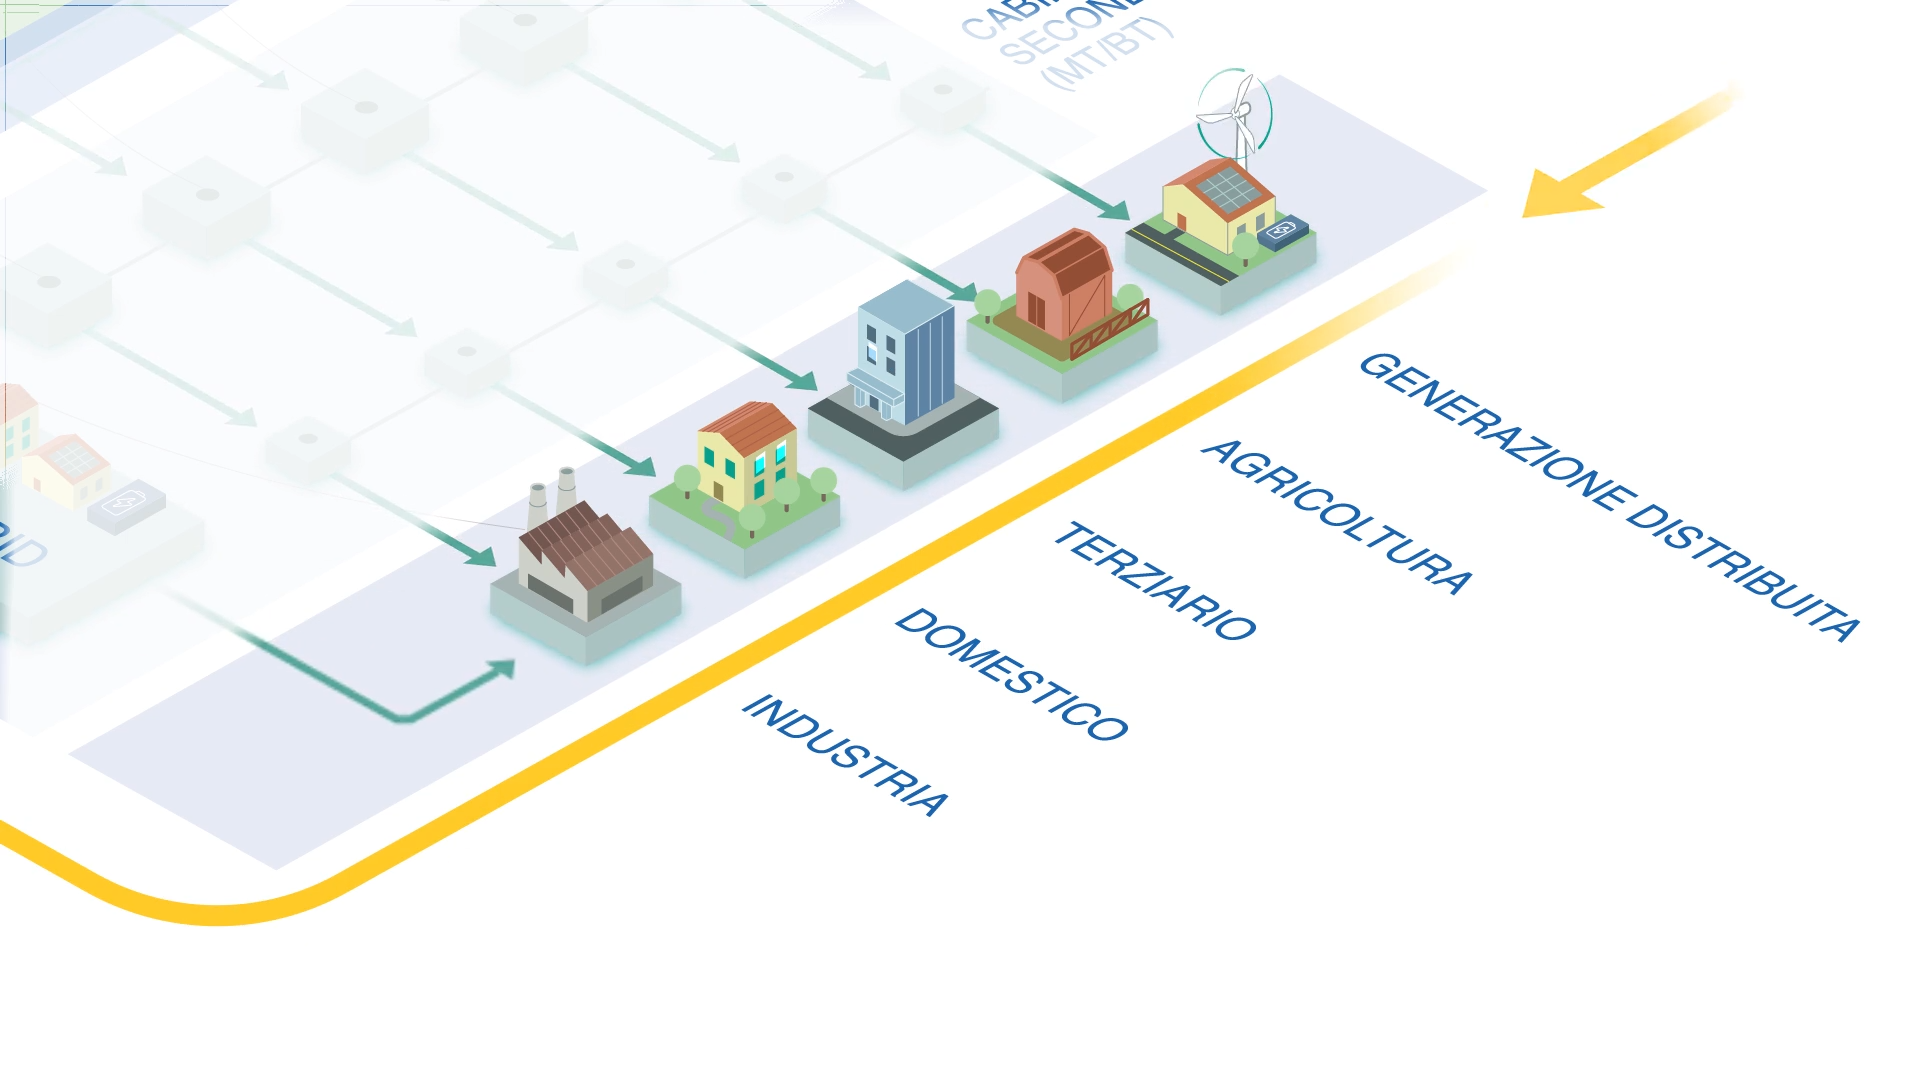
\includegraphics[width=0.5\linewidth]{img/Terna-Utenze.png}
%     \caption{Fonte immagine: Terna - Utenze}
% \end{figure}

%  ---------------------------- FINE AGGEGATO -------------------------------------

\section{Componenti principali della Smart Grid}

La Smart Grid è un'infrastruttura complessa e stratificata, la cui comprensione richiede una scomposizione analitica nei suoi domini funzionali principali. 


Questa sezione si propone di analizzare i componenti fondamentali della Smart Grid, concentrandosi su due aree macroscopiche ma profondamente interconnesse:

\begin{enumerate}
    \item Il \textbf{Dominio del Consumatore} (\textit{Customer Domain}): Rappresenta l'interfaccia diretta tra la rete e l'utente, abilitando una gestione attiva e consapevole dei consumi. Le tecnologie chiave di questo dominio, che verranno analizzate nel dettaglio, includono le Infrastrutture di Misurazione Avanzata (AMI) e i sistemi di gestione energetica domestica (HEMS).

    \item Il \textbf{Dominio Operazionale} (\textit{Operations Domain}): Costituisce il nucleo operativo della rete, responsabile della governance di generazione, trasmissione e distribuzione. In questo ambito operano sistemi di controllo e monitoraggio critici, come le piattaforme SCADA e le tecnologie di misurazione fasoriale (PMU).
\end{enumerate}


La disamina di questi due domini è propedeutica all'identificazione delle superfici di attacco e delle vulnerabilità specifiche di ciascun livello, aspetti centrali per la modellazione delle minacce informatiche oggetto di questa tesi.

\subsection{Dominio del consumatore}

% Questo è il dominio più vicino al cliente ed è composto da:

% \begin{itemize}
%     \item Home/Building Energy Management Systems (\textbf{HEMS/BEMS})
%     \item Advanced Metering Infrastructure (\textbf{AMI})
%     \item Smart Meter (\textbf{SM})
%     \item Data Concentrator (\textbf{DC})
%     \item Head End System (\textbf{HES})
%     \item Meter Data Management System (\textbf{MDMS})
% \end{itemize}



Il Dominio del Consumatore rappresenta il fulcro dell'interazione tra l'utente finale e la Smart Grid. La sua funzione primaria è trasformare il ruolo del consumatore da semplice fruitore passivo di energia a partecipante attivo (\textit{Prosumer}), capace di prendere decisioni informate, gestire i propri carichi e interagire con la rete.


Questo è reso possibile da un ecosistema di tecnologie interconnesse che operano a livello locale, all'interno dell'edificio, e comunicano con i sistemi centrali del DSO. I componenti chiave di questo dominio, che verranno analizzati nei paragrafi seguenti, sono:


\begin{enumerate}
    \item I sistemi di gestione energetica locale, come HEMS e BEMS.
    
    \item L'infrastruttura di comunicazione e misurazione, nota come \textit{Advanced Metering Infrastructure} (AMI), che a sua volta comprende elementi come \textit{Smart Meter} (SM), \textit{Data Concentrator} (DC), \textit{Head-End System} (HES) e \textit{Meter Data Management System} (MDMS).
\end{enumerate}



\subsubsection{Home e Building Energy Management Systems (HEMS/BEMS)}


% Home Energy Managment System (HEMS) o Building Energy Managment System (BEMS), sono dei componenti hardware e software che sono in grado di monitorare il consumo e la produzione degli impianti domestici o di ufficio\footnote{Elettrodomestici, fotovoltaico, HVAC - Heating, Ventilation, e Air Conditioning, batterie di accumulo, autovetture elettriche, antincendio...} e persino controllare dispositivi al fine di consentire un risparmio sulle bollette energetiche e dunque di avere un'edificio più sostenibile \cite{HEMS-SE}.


I sistemi HEMS, per contesti residenziali, e BEMS, per edifici commerciali o terziari, sono piattaforme integrate, composte da hardware e software, progettate per monitorare, analizzare e controllare i flussi energetici all'interno di un edificio \cite{HEMS-SE}.


Le loro funzionalità principali sono:

\begin{itemize}
    \item \textbf{Monitoraggio}: Raccolgono dati in tempo reale sul consumo degli elettrodomestici e sulla produzione di eventuali impianti locali, come ad esempio il fotovoltaico.
    \item \textbf{Controllo e Ottimizzazione}: Consentono di gestire attivamente i carichi, ad esempio posticipando l'avvio di dispositivi ad alto consumo (come lavatrici o veicoli elettrici in carica) nelle fasce orarie più costose o durante i picchi di richiesta della rete.
\end{itemize}


L'obiettivo di questi sistemi è duplice: da un lato, ottimizzare i consumi per generare un risparmio economico per l'utente e aumentare la sostenibilità dell'edificio; dall'altro, abilitare la partecipazione a programmi di \textit{Demand Response} (DR), contribuendo così alla stabilità e all'efficienza della rete elettrica nel suo complesso.


% Un esempio di BEMS, software offerto da Schneider Electric, è \href{https://www.se.com/it/it/work/products/product-launch/building-management-system/}{EcoStruxure™} \footnote{https://www.se.com/it/it/work/products/product-launch/building-management-system/}  che è un architetture integrate che collega i dispositivi all'interno dell'edificio a uno o più Automation Server, gestiti da un software centrale. 
% Questo permette di facilita in modo sicuro lo scambio di dati provenienti sia da Schneider Electric sia da sistemi terzi di gestione dell'energia.

% Un esempio di HEMS, software sempre di Schneider Electric, è \href{https://shop.se.com/us/en}{Schneider Home} \footnote{https://shop.se.com/us/en}.


Un esempio di implementazione in ambito BEMS è la piattaforma \href{https://www.se.com/it/it/work/products/product-launch/building-management-system/}{EcoStruxure™} \footnote{https://www.se.com/it/it/work/products/product-launch/building-management-system/} di Schneider Electric, un'architettura che integra i vari dispositivi e sistemi di un edificio, centralizzandone la gestione. In ambito residenziale, HEMS, la stessa azienda propone soluzioni come \href{https://shop.se.com/us/en}{Schneider Home} \footnote{https://shop.se.com/us/en}.

% , focalizzate sul controllo dei carichi domestici e sull'integrazione con la produzione fotovoltaica e i sistemi di accumulo.


\subsubsection{Advanced Metering Infrastructure (AMI)}

% L'Advanced Metering Infrastructure (AMI) - infrastruttura di misurazione avanzata - è un'evoluzione dell'Automatic Meter Reading (AMR), passando da una lettura unidirezionale e statica ad un sistema bidirezionale e dinamico. La comunicazione può avvenire attraverso reti Wide Area Network (WAN), Neighborhood Area Network (NAN) o Home  Area Network (HAN).


L'AMI rappresenta l'infrastruttura di comunicazione e dati che abilita il dialogo bidirezionale tra l'utente finale e il DSO. Costituisce un'evoluzione cruciale rispetto ai precedenti sistemi di \textit{Automatic Meter Reading} (AMR), che consentivano unicamente la telelettura unidirezionale dei consumi. L'AMI, invece, trasforma il contatore in un \textit{gateway} intelligente, capace di ricevere comandi, inviare dati in tempo quasi reale (\textit{Near Real Time - NRT)} e supportare servizi energetici avanzati.


% Questo sistema permette di raccogliere, memorizzare, analizzare i dati di consumo energetico, fornendo alle aziende che gestiscono la bassa/media tensione la possibilità di monitorare in tempo reale l'utilizzo di elettricità.


% Fanno parte di questa infrastruttura di comunicazione gli Smart Meter (SM), i Data Concentrator (DC), il Head End System (HES) e Meter Data Management System (MDMS). \cite{AMI}


L'architettura AMI è tipicamente stratificata e segue un percorso dati ben definito, che connette il dominio domestico (Home Area Network - HAN) ai sistemi centrali del DSO attraverso reti di quartiere (Neighborhood Area Network - NAN) e reti geografiche estese (Wide Area Network - WAN). Il flusso dei dati coinvolge una catena di componenti specializzati: lo \textit{Smart Meter} (SM), il \textit{Data Concentrator} (DC), l'\textit{Head-End System} (HES) e il \textit{Meter Data Management System} (MDMS) \cite{AMI}.


\subsubsection{Smart Meter (SM)}

% Gli Smart Meter (SM), o più comunemente chiamati Contatori Elettronici (CE), sono quei dispositivi che ogni abitazione, negozio e azienda deve avere per allacciarsi alla rete elettrica.
% Questo dispositivo conta quanti kWh (chilowattora) sono stati consumati da una specifica utenza in un dato periodo e sulla basa di questo il venditore, con cui si ha stipulato il contratto, manderà la fattura da pagare.


Lo SM, o Contatore Elettronico (CE), è il dispositivo terminale dell'architettura AMI, installato presso ogni punto di prelievo (POD) dell'utente finale. Sebbene la sua funzione primaria rimanga la misurazione del consumo energetico, in $kWh$, ai fini della fatturazione, il suo ruolo nella Smart Grid è molto più strategico: esso agisce come un vero e proprio sensore di rete intelligente, un nodo pervasivo capace di raccogliere dati granulari e abilitare servizi avanzati.


% Secondo il D. Lgs. 102/2014 \footnote{https://www.gazzettaufficiale.it/eli/id/2014/07/18/14G00113/sg}, che ha recepito la Direttiva Europea 2012/27/UE sull'efficienza energetica, tutti gli smart meter di prima generazione (1G) dovranno essere sostituiti con dei più moderni CE di seconda generazione (2G) entro il 2035.

% E-Distribuzione ha già completato questa transizione a fine del 2024 \cite{sostituzione-contatori-e-dist}, altri, come Ireti, prevedono di sostituirli completamente entro la fine del 2026 \cite{sostituzione-contatori-Ireti}.

L'evoluzione di questi dispositivi è normata a livello europeo (Direttiva 2012/27/UE) e recepita in Italia dal D. Lgs. 102/2014\footnote{https://www.gazzettaufficiale.it/eli/id/2014/07/18/14G00113/sg}, che ha imposto la sostituzione dei contatori di prima generazione (1G) con i più moderni modelli di seconda generazione (2G). Questa transizione, che E-Distribuzione ha dichiarato conclusa a fine 2024 \cite{sostituzione-contatori-e-dist} e altri DSO come Ireti prevedono di completare entro il 2026 \cite{sostituzione-contatori-Ireti}, non è un semplice aggiornamento tecnologico, ma un cambio di paradigma verso una gestione più attiva e sicura della rete.


% \vspace{0.3cm}
% Il nuovo contatore è stato progettato per essere un
% vero e proprio sensore di rete in grado di misurare tutti i parametri elettrici nel punto di installazione.


\subsubsection{Funzionalità Avanzate dei Contatori di Seconda Generazione CE 2G} 

I contatori 2G introducono un ventaglio di funzionalità innovative che ne espandono notevolmente le capacità. Basandosi sulle specifiche tecniche \cite{chian2-e-dist}\cite{chian2-e-dist-FAQ}\cite{chain2-set-distribuzione}, queste possono essere raggruppate nelle seguenti categorie:

% \begin{itemize}
%     \item Modem Power Line Communication (PLC-banda C CENELEC\footnote{Comitato Europeo di Normalizzazione Elettrotecnica}, 125-140 kHz, con trasmissione almeno pari a 4,8 kbit/s) o Onde Convogliate, protocollo conforme alle norme CEI che consente l'interfacciamento dello SM con dispositivi di lettura del cliente. Commercializzato con il nome di \textit{Chain 2}.
%     \item Supporta un sistema di sicurezza avanzata con autenticazione a cifratura simmetrica AES (Advanced Encryption Standard) con chiavi a 128/256 bit.
%     \item Gestione di processi di autenticazione e crittografia nelle comunicazioni verso i dispositivi utenti
%     \item Back-up del canale primario PLC-banda A, commercializzato con il nome di \textit{Chain 1}\footnote{Canale di comunicazione dedicato che va dal concentratore al contatore utilizzando la rete pubblica GPRS/UMTS/LTE}, su Radio Frequenza (RF) 169 MHz e per l'invio, dai misuratori ai concentratori, di eventi in tempo reale di interruzione/ripristino di tensione.
%     \item Valore massimo di potenza quartoraria giornaliera in prelievo e immissione.
%     \item Disponibilità di misure quantorarie in prelievo e immissione.
%     \item Messaggi personalizzati dal venditore/distributore al cliente.
%     \item Riduzione da remoto della potenza disponibile per clienti morosi.
% \end{itemize}


\begin{enumerate}
    \item \textbf{Comunicazione e Interoperabilità:}
    
    \begin{itemize}
        \item Canale di comunicazione dedicato all'utente, commercializzato con il nome di \textit{Chain 2}: Utilizza la tecnologia \textit{Power Line Communication} (PLC)\footnote{\textit{Power Line Communication} o anche chiamata a Onde Convogliate} in banda C ($125-140\,kHz$)\footnote{PLC-banda C CENELEC, con trasmissione almeno pari a $4,8\, kbit/s$} per dialogare con i dispositivi dell'utente (es. HEMS, \textit{display in-home}), abilitando una reale gestione consapevole dei consumi.
        \item Canale di comunicazione verso il concentratore, \textit{Chain 1}\footnote{Utilizzando la rete pubblica GPRS/UMTS/LTE}: Oltre al canale PLC primario, è previsto un canale di backup su Radio Frequenza (RF) a $169\,MHz$, che garantisce resilienza e permette l'invio in tempo reale di segnalazioni critiche (es. interruzione di tensione).
    \end{itemize}
    
    \item \textbf{Dati e Misure Avanzate:}
    \begin{itemize}
        \item Registrazione delle curve di carico quartorarie: Il contatore registra e rende disponibili i dati di consumo e immissione con una granularità di 15 minuti, permettendo analisi dettagliate e nuovi modelli di tariffazione.
        \item Rilevamento della potenza massima giornaliera: Fornisce dati precisi sui picchi di potenza, utili al DSO per la pianificazione e la gestione della rete.
    \end{itemize}
        \newpage
    \item \textbf{Sicurezza Integrata (\textit{Security by Design}):}
    \begin{itemize}
        \item Crittografia avanzata: Implementa l'algoritmo di cifratura simmetrica \textit{Advanced Encryption Standard} (AES) con chiavi a $128/256$ bit per proteggere la confidenzialità e l'integrità dei dati scambiati sia con il concentratore che con i dispositivi utente.
        \item Autenticazione robusta: Gestisce processi di autenticazione per garantire che solo i dispositivi autorizzati possano comunicare con il contatore.
    \end{itemize}
        
    \item \textbf{Gestione e Controllo Remoto:}
    \begin{itemize}
        \item Modifica remota della potenza: Consente al DSO di variare a distanza la potenza disponibile per l'utente, ad esempio per gestire clienti morosi senza intervento fisico.
        \item Comunicazioni al cliente: Permette al venditore o al distributore di inviare messaggi di testo personalizzati direttamente sul display del contatore.
    \end{itemize}
\end{enumerate}



% \url{https://www.arera.it/fileadmin/allegati/eventi/190522_Sintesi_RSE.pdf}



\subsubsection{Data Concentrator (DC)}

% Il DC, o anche chiamato concentratore, è un altro componente fondamentale per permettere la cosiddetta "Telegestione" infatti consente di trasmettere periodicamente i dati raccolti dagli SM verso i sistemi centrali di monitoraggio del distributore.
% Questa trasmissione avviene attraverso varie tecnologie quali connessioni di rete mobile (GSM, UMTS, LTE e 5G) o, in maniera sempre più diffusa, in fibra ottica. \cite{Comunicazione-con-fornitore-areti}.


% La caratteristica funzionale del concentratore 2G sta nel garantire la retrocompatibilità con CE 1G, introducendo un canale di back-up (RF 169 MHz), del canale primario PLC, o come canale per eventi in termpo reale di interruzione/ripristino di tensione. verso i contatori 2G.\cite{chian2-e-dist}



Il DC, o Concentratore, è un dispositivo intermedio che funge da ponte, \textit{gateway}, tra la NAN e la WAN. Installato tipicamente nelle cabine di trasformazione secondarie (MT/BT), il suo ruolo è cruciale per la scalabilità e l'efficienza dell'infrastruttura AMI. 

Esso aggrega le comunicazioni provenienti da centinaia o migliaia di SM, riducendo il traffico di rete e fungendo da primo livello di elaborazione e gestione dei dati sul campo.

Questo dispositivo è un elemento chiave del sistema di Telegestione, termine che descrive la capacità del DSO di monitorare e comandare la rete di bassa tensione da remoto.

\subsubsection{Caratteristiche e Funzionalità Principali del Concentratore 2G}

Le specifiche tecniche \cite{chian2-e-dist} dei concentratori moderni riflettono il loro duplice ruolo di comunicazione e gestione. Le funzionalità possono essere suddivise come segue:

% \begin{itemize}
%     \item Modem Power Line Communicatiom (PLC) Multi-Modulazione operante in banda A per garantire retrocompatibilità.
%     \item Dotato di Modem di Radio Frequenza per utilizzare il canale 169 MHz come back-up del canale PLC per la comunicazione verso i contatori 2G.
%     \item Consente l’invio in tempo reale al sistema centrale di eventi di assenza e ripristino tensione dell'apparato e rete BT associata e del contatore 2G.
%     \item Consente la raccolta massiva dei picchi di potenza massima giornaliera.
%     \item Supporta una connessione 3G/4G per le comunicazioni verso il sistema centrale e una porta ethernet per un collegamento a un router di cabina MT/BT.
%     \item Supporta la cifratura del canale di comunicazione da concentratore a sistema centrale secondo standard internazionali.
% \end{itemize}

\begin{enumerate}
    \item \textbf{Comunicazione con gli Smart Meter (Interfaccia NAN):}
    \begin{itemize}
        \item[--] Supporto Multi-Tecnologia: È dotato di modem PLC multi-modulazione, operante in banda A per garantire la retrocompatibilità con i contatori di prima generazione (1G), e di modem RF a $169\,MHz$ per comunicare con i contatori 2G, utilizzando quest'ultimo anche come canale di backup.
    \end{itemize}
    
    \item \textbf{Comunicazione con il Sistema Centrale (Interfaccia WAN):}
    \begin{itemize}
        \item[--] Connettività Resiliente: Supporta molteplici canali di comunicazione verso l'Head-End System, inclusa la connettività mobile (3G/4G/5G) e una porta Ethernet per il collegamento a router in fibra ottica, garantendo alta affidabilità \cite{Comunicazione-con-fornitore-areti}.
        \item[--] Sicurezza del Canale: Implementa la cifratura del canale di comunicazione verso il sistema centrale secondo standard internazionali, assicurando la confidenzialità e l'integrità dei dati aggregati.
    \end{itemize}
    
    \item \textbf{Gestione dei Dati e degli Eventi:}
    \begin{itemize}
        \item[--] Raccolta Massiva e Aggregazione: È programmato per raccogliere in modo massivo i dati di misura (es. curve di carico, picchi di potenza) dagli Smart Meter e aggregarli prima dell'invio.
        \item[--] Gestione di Eventi in Tempo Reale: Rileva e inoltra immediatamente al sistema centrale eventi critici provenienti dalla rete di bassa tensione, come l'assenza o il ripristino della tensione su un contatore 2G, permettendo al DSO di reagire prontamente a guasti o anomalie.
    \end{itemize}
\end{enumerate}


\subsubsection{Head End System (HES)}

% L'Head-End System (HES) è uno dei componenti fondamentali dell'AMI e funge da interfaccia principale tra i sistemi centrali dell'azienda e la vasta rete di contatori intelligenti e concentratori di dati distribuiti sul territorio.



% Modulo di Head End finalizzato alla gestione della comunicazione con gli apparati connessi alla rete di bassa/medi/alta tensione (contatori, concentratori) per l’acquisizione remota di dati di misura ed eventi e l’esecuzione delle attività di telegestione. Questo modulo è cruciale in quanto deve garantire le performance richieste nella deliberazione 87/2016, sia in termini di volumi sia di tempistiche, e richiede soluzioni a elevata scalabilità, garantibili soltanto mediante l’utilizzo di soluzioni in cloud. \cite{chian2-e-dist-2017}


% L'HES rappresenta un elemento cardine dell'infrastruttura AMI, operando come interfaccia strategica tra i sistemi centrali aziendali e l'ecosistema distribuito di contatori intelligenti e concentratori di dati presenti sul territorio.


% Questo modulo specializzato gestisce integralmente la comunicazione con tutti gli apparati connessi alla rete elettrica di bassa, media e alta tensione, includendo contatori e concentratori. Le sue funzioni principali comprendono l'acquisizione remota di dati di misura ed eventi, nonché l'esecuzione delle attività di telegestione degli impianti.


% Il sistema HES riveste un ruolo critico nel garantire il rispetto dei parametri prestazionali stabiliti dalla deliberazione 87/2016\footnote{Delibera 08 marzo 2016
% 87/2016/R/eel - https://www.arera.it/atti-e-provvedimenti/dettaglio/16/87-16}, sia per quanto riguarda i volumi di dati processati che le tempistiche di risposta. Per soddisfare questi requisiti stringenti, è necessario implementare soluzioni caratterizzate da elevata scalabilità, obiettivo raggiungibile efficacemente solo attraverso l'adozione di architetture cloud native. \cite{chian2-e-dist-2017}


L'HES è il cuore software dell'infrastruttura AMI. Esso funge da interfaccia strategica, un \textit{gateway} centralizzato che media la comunicazione tra i sistemi informativi aziendali del DSO e l'intero ecosistema di dispositivi distribuiti sul campo, ovvero i DC e, attraverso di essi, gli SM.


Il suo ruolo è quello di orchestrare e gestire tutte le interazioni con la rete di misurazione. 
Le sue funzioni principali possono essere sintetizzate come segue:


\begin{itemize}
    \item \textbf{Gestione delle Comunicazioni:} Stabilisce, mantiene e protegge le sessioni di comunicazione con migliaia di DC simultaneamente.
    \item \textbf{Acquisizione Dati e Telegestione:} Esegue le operazioni di lettura massiva dei dati di misura (curve di carico, eventi) e invia comandi di telegestione verso i dispositivi periferici (es. aggiornamenti firmware, modifiche contrattuali, comandi di Demand Response).
    \item \textbf{Validazione e Normalizzazione:} Riceve i dati "grezzi" dal campo, li valida per verificarne la correttezza formale e li normalizza in un formato standardizzato, pronto per essere inoltrato ai sistemi di livello superiore.
\end{itemize}


L'HES ha un'importanza critica nel garantire il rispetto dei rigorosi parametri prestazionali imposti dalla normativa, come la delibera ARERA 87/2016 \footnote{Delibera 08 marzo 2016 87/2016/R/eel - https://www.arera.it/atti-e-provvedimenti/dettaglio/16/87-16}, in termini di volumi di dati processati e tempistiche di risposta. Per soddisfare tali requisiti, le implementazioni moderne di HES devono essere caratterizzate da un'elevata scalabilità e affidabilità. Questo obiettivo, come evidenziato in \cite{chian2-e-dist-2017}, è raggiungibile in modo efficace principalmente attraverso l'adozione di architetture cloud-native, un aspetto che espone questi sistemi a specifici vettori di minacce informatiche.


\subsubsection{Meter Data Management System (MDMS)}

% Il Meter Data Management System (MDMS) è un altro componente fondamentale che permette al distributore di energia di ricevere i dati dei DC, soprattutto grazie all'HES. In questa fase i dati vengono:


L'MDMS è la piattaforma software di back-end che agisce come repository centrale e motore analitico per tutti i dati di misura raccolti dall'infrastruttura AMI. Una volta che l'HES ha acquisito e normalizzato i dati provenienti dal campo, li inoltra all'MDMS, che diventa la "\textit{single source of truth}" (unica fonte di verità) per tutte le informazioni relative ai consumi e allo stato della rete di bassa tensione.


Il ciclo di vita del dato all'interno dell'MDMS si articola in diverse fasi cruciali:

% \begin{itemize}
%     \item Validati, stimati e modificati
%     \item Memorizzati e archiviati in maniera sicura per il lungo termine
%     \item Analizzati e aggregati per creare profili di carico, previsione futura e calcolo dei fattori determinanti per la fatturazione
%     \item Condivisi e strutturati per altri sistemi di utilità. In particolar modo il Distribution Management System (DMS) può gestire i dati aggregati per gestire la rete a media/bassa tensione, mentre  Energy Management System (EMS) per gestire la rete ad alta tensione e la generazione di energia.
% \end{itemize}

\begin{enumerate}
    \item \textbf{Validazione, Stima e Modifica} (VEE - \textit{Validation, Estimation, and Editing}): I dati grezzi vengono sottoposti a un processo rigoroso di VEE per identificare anomalie, correggere valori mancanti o palesemente errati attraverso algoritmi di stima, e preparare un \textit{dataset} pulito e affidabile.
    
    \item \textbf{Archiviazione a Lungo Termine}: I dati validati vengono memorizzati e archiviati in modo sicuro, garantendo la loro disponibilità per analisi storiche, dispute di fatturazione e obblighi normativi. La gestione dell'Alta Affidabilità (HA) e del \textit{Disaster Recovery} (DR) di questi dati critici è spesso affidata ai meccanismi nativi delle piattaforme cloud su cui questi sistemi sono implementati.
    
    \item \textbf{Analisi e Aggregazione}: L'MDMS aggrega i dati granulari per creare profili di carico, eseguire previsioni sui consumi futuri (\textit{forecasting}) e calcolare i dati necessari per i processi di fatturazione.
    
    \item \textbf{Integrazione e Condivisione}: Agisce come un hub centrale che espone i dati elaborati, in formati strutturati, ad altri sistemi aziendali critici. Ad esempio, fornisce dati aggregati al \textit{Distribution Management System} (DMS) per ottimizzare le operazioni sulla rete di media/bassa tensione, o all'\textit{Energy Management System} (EMS) per analisi a livello di rete di trasmissione.
\end{enumerate}


% La gestione degli aspetti di Alta Affidabilità (HA) e Disaster Recovery (DR) viene affidata agli strumenti nativi messi a disposizione dalla piattaforma cloud adottata, garantendo così robustezza operativa senza compromettere la semplicità architetturale né l'efficienza complessiva della soluzione.


% Per abilitare la comunicazione bidirezionale tra il sistema centrale BEAT e i dispositivi distribuiti sul campo, i concentratori di nuova generazione integrano modem cellulari con connettività 3G/4G e relative schede SIM dedicate.


% Dal punto di vista della sicurezza informatica, la rete mobile risulta protetta attraverso un'architettura segregata che implementa controlli firewall granulari per la gestione delle autorizzazioni di accesso. Questa configurazione assicura che ogni tentativo di connessione venga sottoposto a preventiva validazione e autorizzazione prima di consentire l'accesso alle risorse di sistema. \cite{chian2-e-dist-2017}

In sintesi, se l'HES è il "motore" della comunicazione, l'MDMS è il "cervello" analitico che trasforma la mole di dati grezzi in informazioni di valore, abilitando decisioni operative e strategiche sia per il DSO che il TSO.


\begin{figure}[h!]
    \centering
    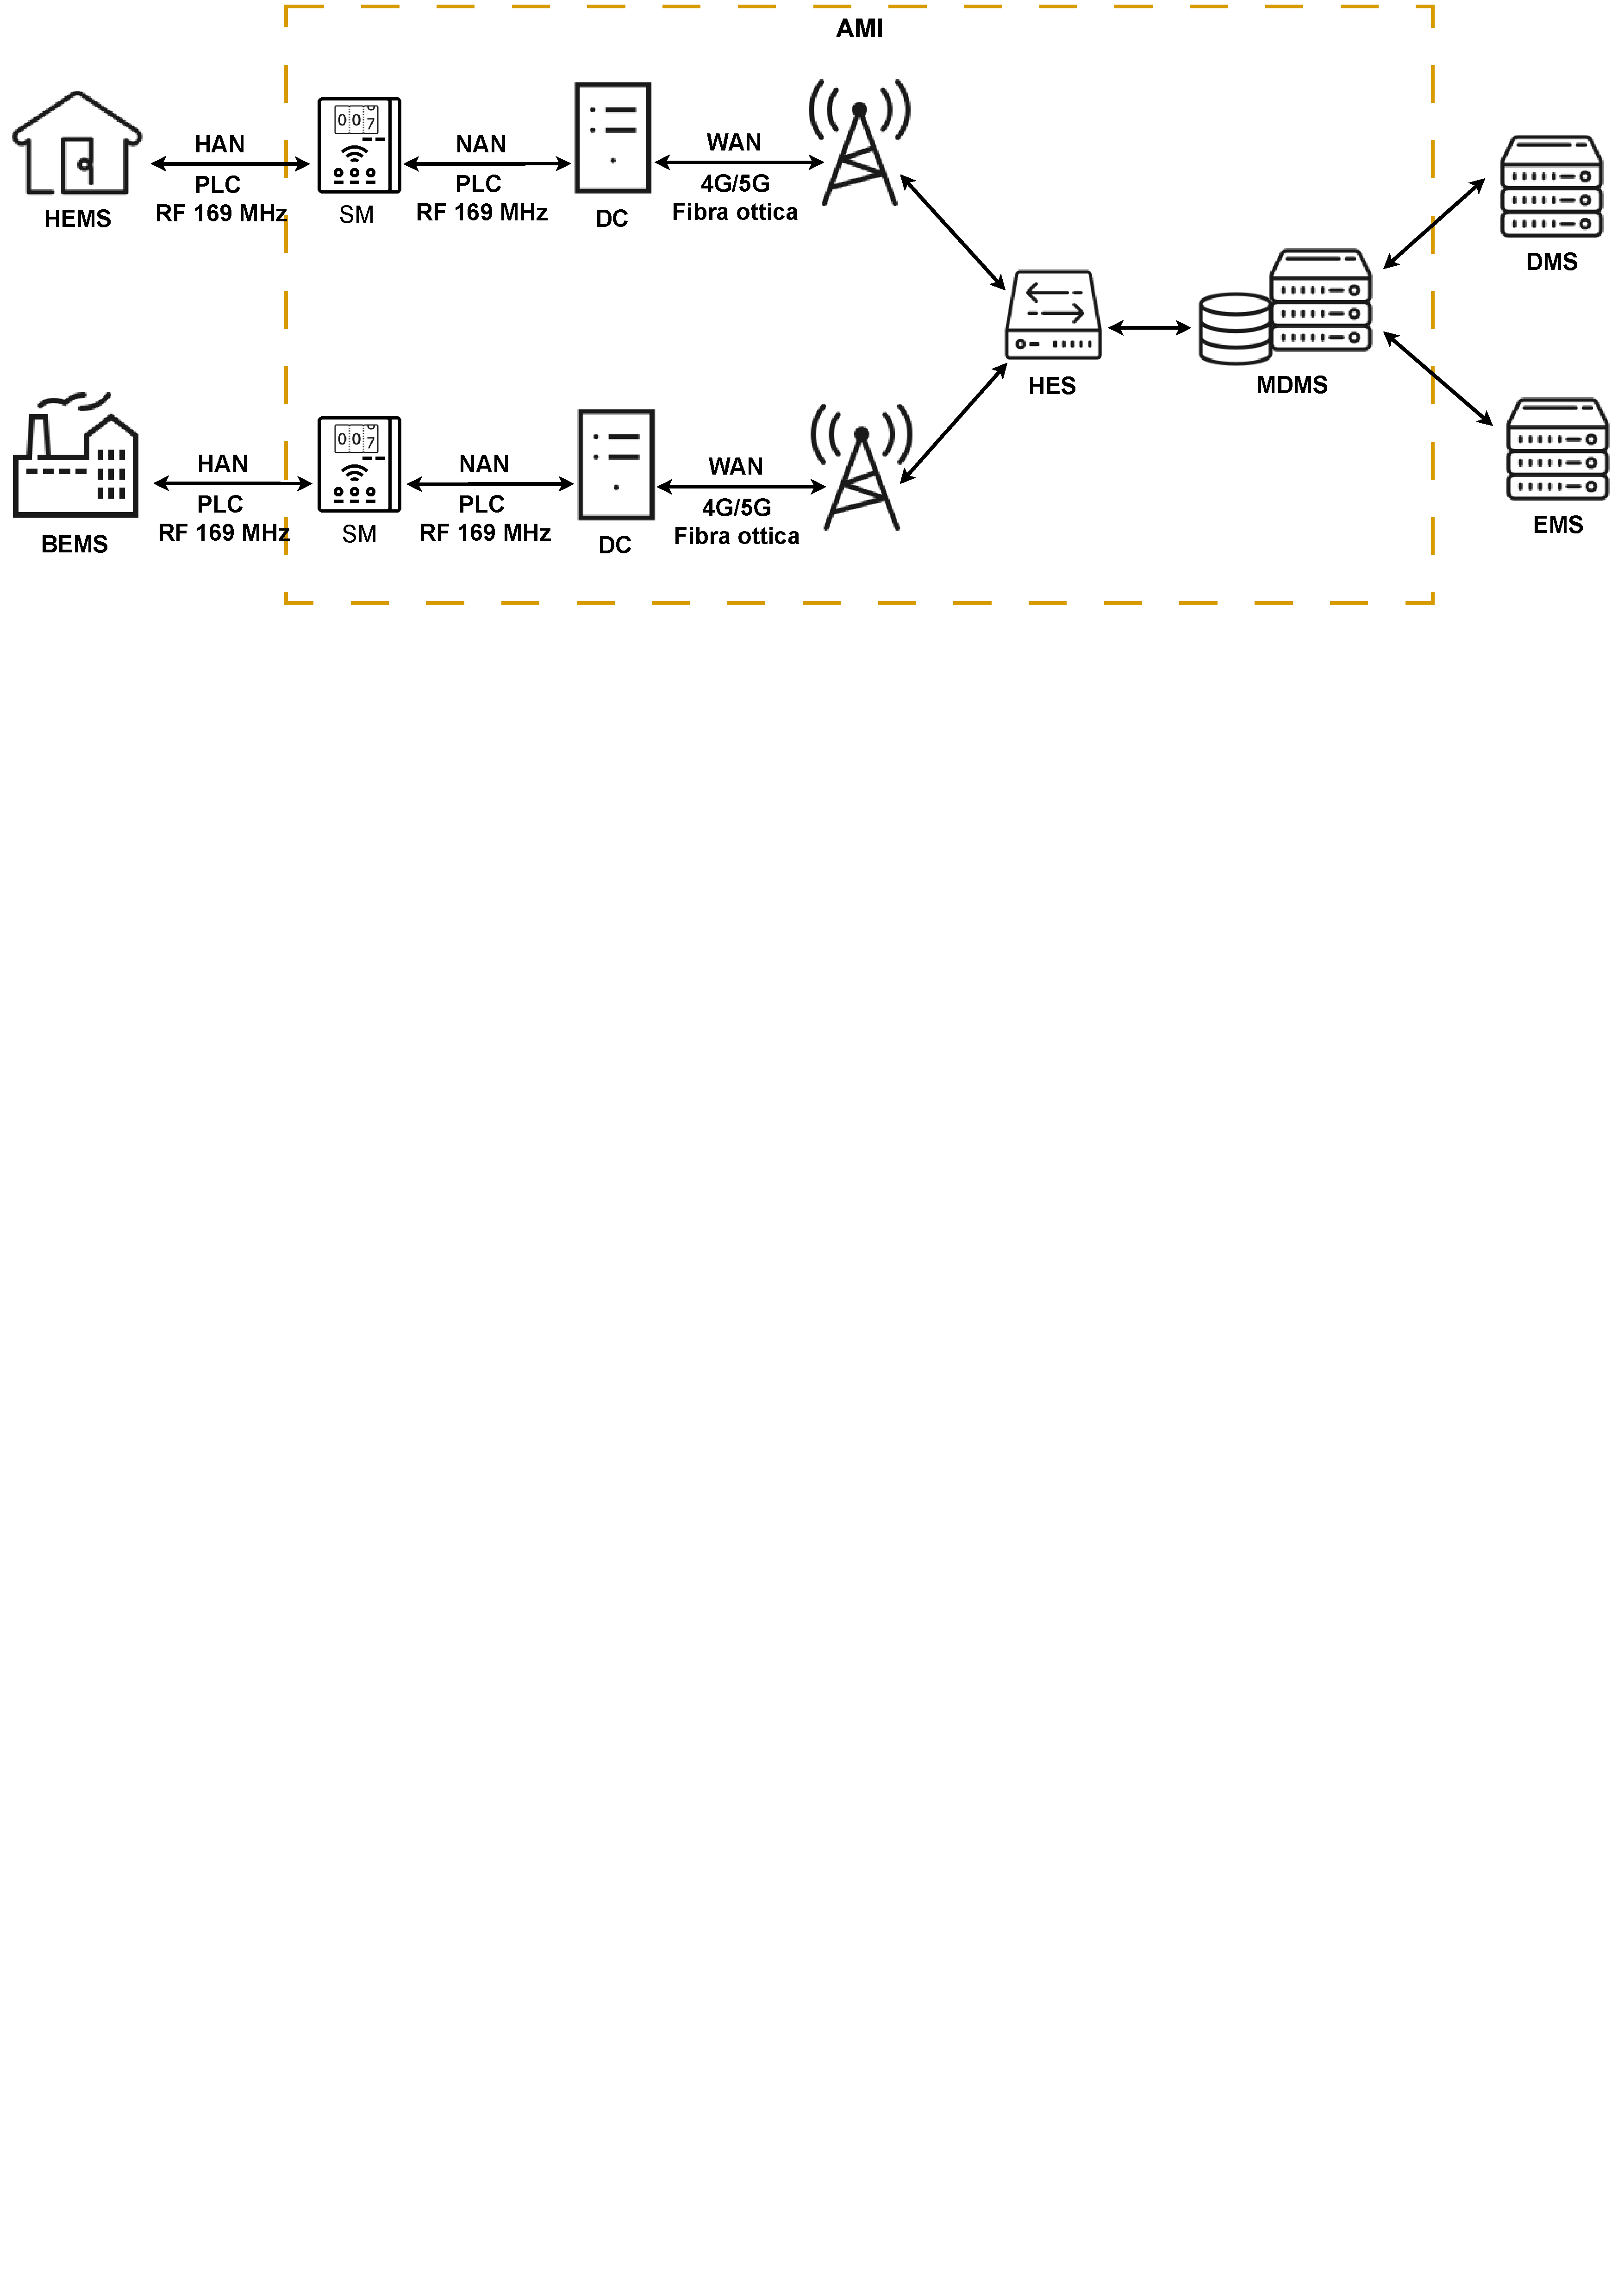
\includegraphics[trim= 0cm 61cm 0cm 0cm, clip, width=0.9\linewidth]{img/client-view-v2.drawio.pdf}
    \caption{Dominio del consumatore}
\end{figure}





\subsection{Dominio operazionale}

% Questo è il dominio più operativo principalmente gestito dal Transmission System Operator (TSO), Terna, ed è composto da:

% \begin{itemize}
%     \item Phasor Measurement Units (\textbf{PMU})
%     \item Phasor Data Concentrator (\textbf{PDC})
%     \item Energy Management System (\textbf{EMS})
%     \item Distribution Management System (\textbf{DMS})
%     \item Supervisory Control and Data Acquisition (\textbf{SCADA})
%     \item Generation Management System (\textbf{GMS})
%     \item Remote Terminal Units (\textbf{RTU})
%     \item Intelligent Electronic Devices (\textbf{IED})
% \end{itemize} 


Il Dominio Operazionale rappresenta il centro di controllo nevralgico della Smart Grid, l'insieme dei sistemi e delle tecnologie responsabili della gestione, del monitoraggio e della protezione dell'infrastruttura fisica di generazione, trasmissione e distribuzione dell'energia.


A differenza del Dominio del Consumatore, focalizzato sull'utente finale, questo dominio è di competenza esclusiva degli operatori di rete: il TSO per la rete di alta e altissima tensione e il DSO per le reti di media e bassa tensione.


L'obiettivo di questo dominio è garantire che l'energia sia prodotta, trasportata e consegnata in modo stabile, efficiente e sicuro, mantenendo in ogni istante l'equilibrio tra domanda e offerta. Per raggiungere questo scopo, si avvale di una complessa architettura tecnologica, i cui componenti principali possono essere raggruppati in tre categorie funzionali:



% \begin{enumerate}
%     \item Sistemi di Monitoraggio Sincronizzato (WAMS): tecnologia utile per una visione in tempo reale dello stato della rete, basata su:
%     \begin{itemize}
%         \item \textit{Phasor Measurement Unit} (PMU)
%         \item \textit{Phasor Data Concentrator} (PDC)
%     \end{itemize}
    
%     \item Sistemi di Gestione Avanzata: le piattaforme software di alto livello per l'ottimizzazione e la gestione della rete, che includono:
%     \begin{itemize}
%         \item \textit{Energy Management System} (EMS) per la rete di trasmissione.
%         \item \textit{Distribution Management System} (DMS) per la rete di distribuzione.
%         \item \textit{Generation Management System} (GMS) per la programmazione della generazione.
%     \end{itemize}
    
%     \item Sistemi di Controllo e Acquisizione Dati (SCADA): la spina dorsale del controllo operativo, composta da:
%     \begin{itemize}
%         \item \textit{Supervisory Control and Data Acquisition} (SCADA)
%         \item Dispositivi di campo come \textit{Remote Terminal Unit} (RTU) e \textit{Intelligent Electronic Device} (IED)
%     \end{itemize}
% \end{enumerate}

\begin{enumerate}
    \item Sistemi di Monitoraggio Sincronizzato (WAMS): tecnologia utile per una visione in tempo reale dello stato della rete, basata su: \textit{Phasor Measurement Unit} (PMU) e \textit{Phasor Data Concentrator} (PDC)
    
    \item Sistemi di Gestione Avanzata: le piattaforme software di alto livello per l'ottimizzazione e la gestione della rete, che includono:
    \textit{Energy Management System} (EMS) per la rete di trasmissione,  il \textit{Distribution Management System} (DMS) per la rete di distribuzione e \textit{Generation Management System} (GMS) per la programmazione della generazione.
    
    \item Sistemi di Controllo e Acquisizione Dati (SCADA): la spina dorsale del controllo operativo, composta da: \textit{Supervisory Control and Data Acquisition} (SCADA) e dispositivi di campo come \textit{Remote Terminal Unit} (RTU) e \textit{Intelligent Electronic Device} (IED).
\end{enumerate}


Nei paragrafi seguenti, ciascuno di questi componenti verrà analizzato nel dettaglio per comprenderne il ruolo specifico e le interazioni all'interno dell'architettura operativa.



\subsubsection{Phasor Measurement Units (PMU)}

% I Phasor Measurement Units (PMU), unità di misuramento del fasore, è un sensore estremamente preciso che riesce a controllare la fase e l'ampiezza della sinusoide di rete, ma soprattutto deve essere dotato di una sincronizzazione temporale molto accurata.

% Per quest'ultimo scopo si ricorre al protocollo IEEE 1588 PTP (Precision Time Protocol) oppure GPS che consente la misurazione sincronizzata in tempo reale di più punti remoti della rete.

% Queste misurazioni sincronizzate nel tempo sono importanti perché se la domanda e l'offerta della rete non sono perfettamente sincronizzate, gli squilibri di frequenza possono causare uno stress sulla rete, che è una potenziale causa di interruzioni di corrente.

% \vspace{0.3cm}

% Questi dispositivi sono principalmente utilizzati nella rete ad alta e altissima tensione e sono sparsi su tutta la Rete di Trasmissione Nazionale (RTN). 

% in https://download.terna.it/terna/Capitolo%201_Nuova%20sezione%201C_8d787c66135589d.pdf a pagina 47 si parla che i PMU devono essere posti in corrispondenza di generatori di 50 MVA  (GIà IN BIBLIOGRAFIA \cite{Fase-di-rete}.


% Il Phasor Measurement Units (PMU), unità di misuramento del fasore, è un dispositivo di misura avanzato che rileva in tempo reale il fasore di rete con elevata precisione temporale.
% Per quest'ultimo scopo si ricorre al protocollo IEEE 1588 PTP (Precision Time Protocol) oppure GPS che consente di confrontare i valori misurati (sincrofasori) da diverse sottostazioni distanti tra loro e di trarre conclusioni sullo stato del sistema e su eventi dinamici come le condizioni di oscillazione della potenza. \cite{siemens-PMU}

% Queste misurazioni sincronizzate nel tempo sono importanti perché se la domanda e l'offerta della rete non sono perfettamente sincronizzate, gli squilibri di frequenza possono causare uno stress sulla rete, che è una potenziale causa di interruzioni di corrente.

Il PMU, o unità di misura fasoriale, è un dispositivo di monitoraggio avanzato che rileva in tempo reale i fasori di tensione e corrente della rete elettrica. La caratteristica distintiva del PMU è la sua capacità di associare a ogni misura un marcatore temporale (\textit{timestamp}) di altissima precisione, ottenuto tramite segnali di sincronizzazione da GPS o protocolli di rete come il \textit{Precision Time Protocol} (PTP - IEEE 1588) \cite{siemens-PMU}.


Questa sincronizzazione temporale permette di confrontare istantaneamente le misure provenienti da punti diversi e geograficamente distanti della rete, creando una fotografia dinamica e coerente dello stato del sistema. I dati così ottenuti, noti come sincrofasori, sono fondamentali per analizzare fenomeni dinamici come le oscillazioni di potenza e per prevenire instabilità. Infatti, un disallineamento fasoriale tra diverse aree della rete è un indicatore precoce di stress sistemico, che, se non gestito, può portare a disservizi o blackout.


% I PMU sono fondamentali per:

% \begin{itemize}
%     \item Monitoraggio dello stato della rete in tempo reale
%     \item Analisi della stabilità del sistema
%     \item Rilevamento rapido di disturbi o anomalie
%     \item Supporto alle procedure di protezione e controllo
% \end{itemize}

I PMU sono i sensori alla base dei \textit{Wide Area Monitoring Systems} (WAMS), sistemi di monitoraggio ad area estesa che offrono una visibilità in tempo reale sullo stato della rete. Grazie ai dati forniti dai PMU, gli operatori di rete possono:


\begin{itemize}
    \item Eseguire un'analisi della stabilità del sistema in tempo reale.
    \item Rilevare con estrema rapidità l'insorgere di disturbi e anomalie.
    \item Migliorare l'efficacia delle procedure di protezione e controllo della rete.
\end{itemize}



% Questi dispositivi sono principalmente utilizzati nella rete ad alta e altissima tensione e sono sparsi su tutta la Rete di Trasmissione Nazionale (RTN), oltre ad essere utilizzati anche negli impianti di generazione di taglia superiore o uguale a $50\,MVA$ \cite{Fase-di-rete}. Questa soglia identifica gli impianti di taglia significativa che possono influenzare in modo rilevante il sistema elettrico.

% I PMU sono principalmente utilizzati nella Rete di Trasmissione Nazionale (RTN) ad alta (AT) e altissima tensione (AAT), oltre ad essere utilizzati anche negli impianti di generazione di taglia superiore o uguale a $50\,\text{MVA}$ in corrispondenza delle sbarre di AT della stazione di consegna \cite{Fase-di-rete-terna}. Questa soglia identifica gli impianti di taglia significativa che possono influenzare in modo rilevante il sistema elettrico.


% Oltre ad essere utilizzati nella RTN ad Alta ed Altissima Tensione, dove il loro costo elevato è giustificato dall'importanza critica del monitoraggio di sistema, i PMU possono anche essere utilizzati dai distributori per monitorare la MT/BT, soprattutto in un contesto di Smart Grid con elevata immissione di energia rinnovabile da parte dei piccoli produttori con impianti domestici, benché l'investimento economico richiesto ne limiti attualmente la diffusione capillare nelle reti di distribuzione e perché i fenomeni di instabilità sono generalmente localizzati e di minor intensità.


Data la loro importanza strategica e il costo, i PMU sono installati prevalentemente nella Rete di Trasmissione Nazionale (RTN), su linee AT/AAT, e nei punti di connessione degli impianti di generazione di taglia significativa, $\geq 50\,\text{MVA}$, dove l'impatto sul sistema è maggiore \cite{Fase-di-rete-terna}. Sebbene il loro impiego nelle reti di distribuzione (MT/BT) sia tecnicamente possibile e potenzialmente utile per gestire l'intermittenza delle fonti rinnovabili distribuite (DER), la loro diffusione in questo ambito è attualmente limitata da considerazioni economiche e dalla natura più localizzata dei fenomeni di instabilità a questo livello.


\subsubsection{Phasor Data Concentrator (PDC)}

% Il PDC possiede capacità computazionale per collezionare ed aggregare i dati rilevati dai PMU e potenzialmente altri PDC, per poi inviarli ad altri sistemi quali ad esempio gli Energy Management System (EMS), Supervisory Control and Data Acquisition (SCADA) e altri. Dunque non solo concentra e allinea i dati da varie sorgenti, ma offre anche capacità avanzate di elaborazione, conversione e monitoraggio, interagendo con un ampio spettro di dispositivi e applicazioni per supportare il monitoraggio.


% I PDC possono comunicare attraverso vari canali di comunicazione, tra cui reti seriali e/o Ethernet, supportando appunto protocolli per la comunicazione generale come TCP (Transmission Control Protocol) e UDP (User Datagram Protocol) e gli standard IPv4 e IPv6.

% Supporta vari protocolli di trasferimento dei dati sincrofasori, come IEEE Std C37.118.2-2011, IEEE Std C37.118-2005, IEEE Std 1344-1995 e IEC 61850-90-5. Questo consente a un PDC di ricevere, interpretare e trasmettere dati nel protocollo supportato. Come minimo, un PDC deve supportare la ricezione, il parsing, l'interpretazione e l'invio di dati in conformità con almeno un protocollo per trasferimento dei sincrofasori.\cite{IEEE-article-PDC}

Il PDC è il componente centrale dell'architettura WAMS, agendo come nodo di aggregazione e sincronizzazione per i flussi di dati provenienti dai PMU. La sua funzione primaria è quella di raccogliere i dati dei sincrofasori da molteplici PMU, allinearli temporalmente in un unico \textit{dataset} coerente e inoltrarli ai sistemi di gestione di livello superiore, come l'EMS o piattaforme SCADA avanzate.


I PDC sono spesso organizzati in un'architettura gerarchica: PDC di livello inferiore possono raccogliere dati direttamente dalle PMU, mentre PDC di livello superiore (o "Super PDC") aggregano i dati provenienti da altri PDC, permettendo una visione consolidata di intere regioni o dell'intera rete nazionale \cite{PDC}. Figura \ref{comunicaizone-pdc}.


Le capacità di un PDC possono essere riassunte nelle seguenti funzioni chiave:

\begin{itemize}
    \item \textbf{Aggregazione e Sincronizzazione Dati:} Colleziona flussi di dati da più fonti, li ordina in base al loro timestamp e crea un set di dati unico e cronologicamente coerente, essenziale per un'analisi accurata dello stato della rete.
    \item \textbf{Elaborazione e Monitoraggio in Tempo Reale:} Oltre all'aggregazione, i PDC moderni possono eseguire calcoli e analisi in tempo reale sui dati ricevuti (es. controllo della qualità dei dati, rilevamento di eventi), fornendo riscontri immediati agli operatori.
    \item \textbf{Garanzia di Interoperabilità:} Un ruolo cruciale del PDC è quello di garantire l'interoperabilità tra dispositivi di diversi fornitori. Per questo, supporta una vasta gamma di protocolli standardizzati per il trasferimento dei sincrofasori, tra cui IEEE C37.118 (nelle sue varie revisioni) e IEC 61850-90-5. Questo permette al PDC di ricevere, interpretare e, se necessario, convertire dati tra diversi formati \cite{IEEE-article-PDC}.
    \item \textbf{Comunicazione Robusta:} Per la trasmissione dei dati, i PDC utilizzano canali di comunicazione affidabili, tipicamente basati su reti Ethernet e protocolli standard come TCP/IP (sia IPv4 che IPv6), assicurando una connettività sicura e performante verso i sistemi centrali.
\end{itemize}


\begin{figure}[h]
    \centering
    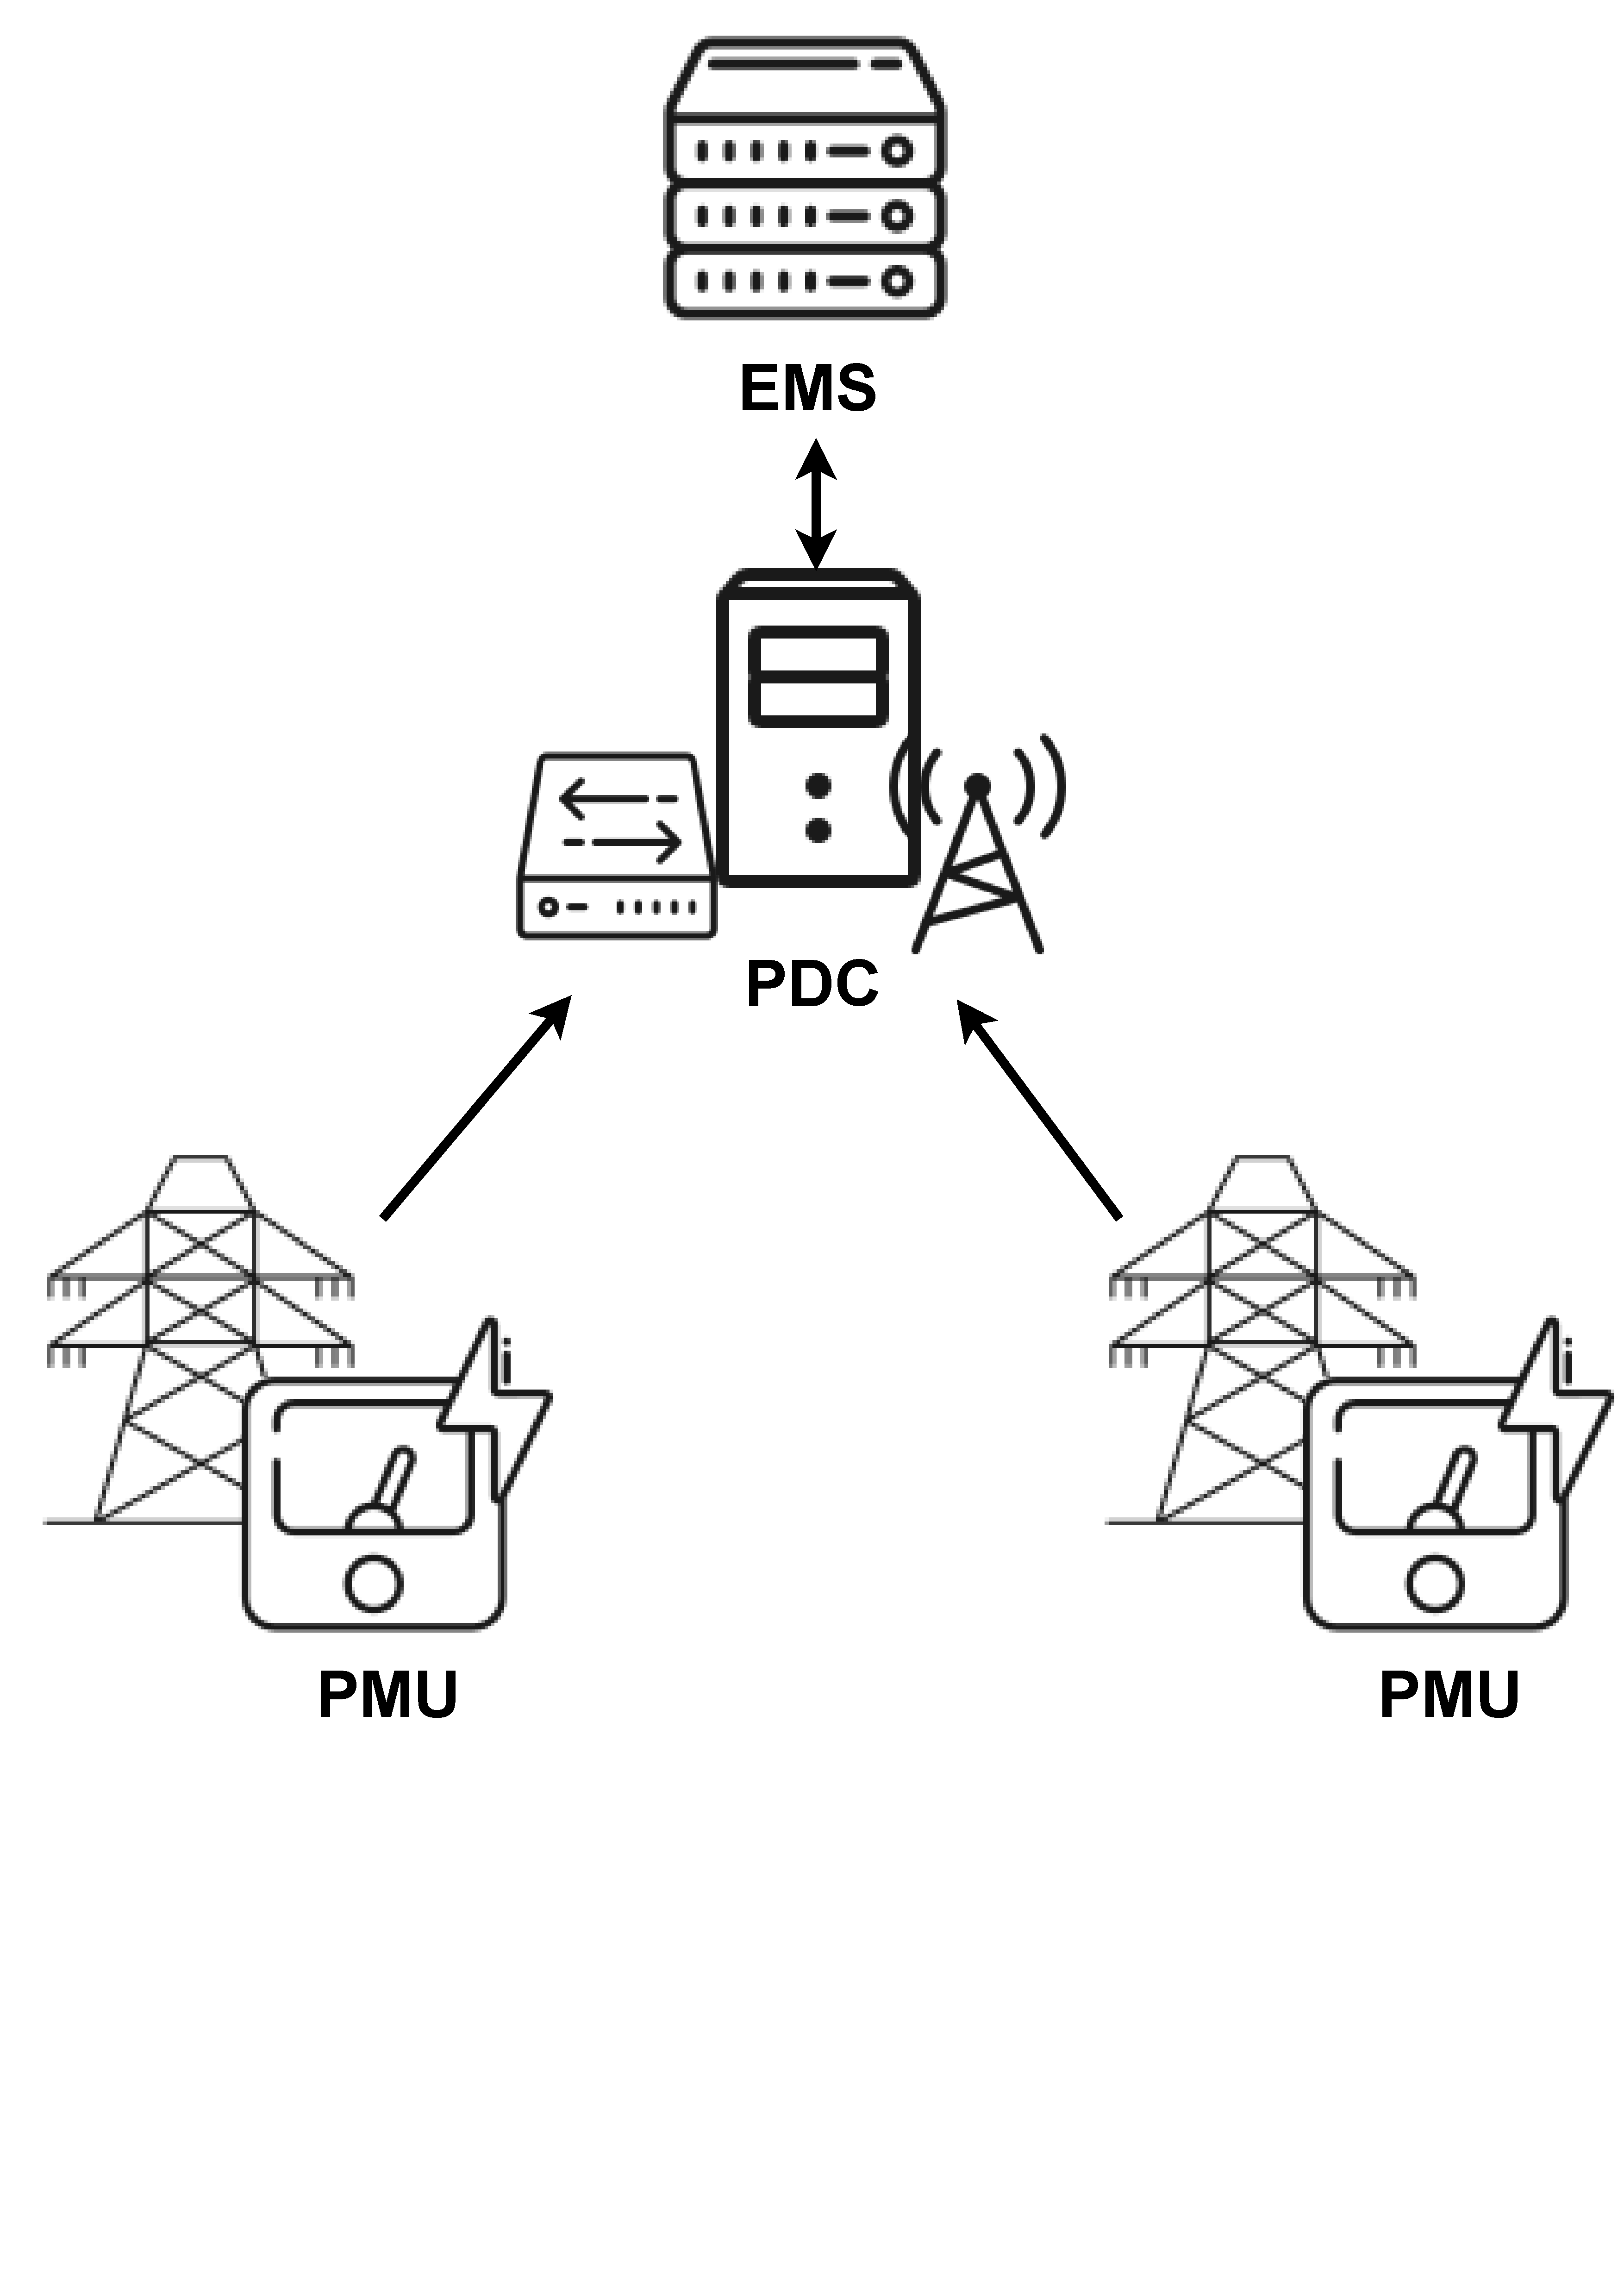
\includegraphics[trim= 0cm 20cm 0cm 0cm, clip, width=0.4\linewidth]{img/PMU-connection-v2.drawio.pdf}
    \caption{Esempio di connessione tra PMU e PDC \cite{PDC}}
    \label{comunicaizone-pdc}
\end{figure}


\newpage
\subsubsection{Energy Management System (EMS)}


% Una funzione chiave dell'Energy Management System (EMS)\footnote{In questo contento si può parlare anche di Utility Energy Management Systems (UEMS) - destinato alle aziende di servizi pubblici che si concentrano a livello di distribuzione e trasmissione dell'energia di rete.}, posto in un contesto di AT e AAT, è quella di garantire che l'elettricità sia generata e distribuita nel modo più efficiente ed economico possibile.\cite{EMS-GE}

% Questo include:

% \begin{itemize}
%     \item Bilanciare la domanda e l'offerta: Il sistema EMS lavora costantemente per far coincidere la produzione di elettricità con il consumo, il che è fondamentale per mantenere la stabilità della rete.
    
%     \item Integrare le energie rinnovabili: Con l'aumento delle fonti energetiche rinnovabili intermittenti come l'eolico e il solare, il sistema di gestione ambientale è essenziale per gestire la loro variabilità. Può, ad esempio, prevedere la produzione di energia da queste fonti e regolare di conseguenza altre centrali elettriche o sistemi di stoccaggio dell'energia.
    
%     \item Dispacciamento economico: L'EMS aiuta a determinare il modo più economico di generare elettricità in un dato momento, considerando fattori come il costo del carburante e l'efficienza dell'impianto.
% \end{itemize}



% Come si può intuire, l'EMS è un'infrastruttura critica che combina l'acquisizione di dati da varie fonti, quali ad esempio i sistemi SCADA, il monitoraggio in tempo reale e l'analisi avanzata per consentire sia il controllo automatizzato che il processo decisionale "human-in-the-loop" per il funzionamento sicuro, affidabile ed efficiente della rete elettrica ad alta ed altissima tensione. \cite{enelx-EMS}



L'EMS\footnote{In questo contento si può parlare anche di Utility Energy Management Systems (UEMS) - destinato alle aziende di servizi pubblici che si concentrano a livello di distribuzione e trasmissione dell'energia di rete.} è la piattaforma software di alto livello che funge da "cervello" operativo e decisionale per la gestione della rete di trasmissione, AT e AAT. Mentre i sistemi SCADA si occupano primariamente dell'acquisizione dati e del controllo in tempo reale dei singoli apparati, l'EMS opera a un livello superiore: utilizza i dati provenienti da SCADA, PMU e altre fonti per eseguire analisi complesse e applicazioni di ottimizzazione, con l'obiettivo di garantire una gestione della rete sicura, affidabile ed economicamente efficiente \cite{enelx-EMS, EMS-GE}.

Le funzioni strategiche di un EMS sono finalizzate al mantenimento costante dell'equilibrio tra generazione e carico. Tra le sue principali responsabilità si includono:


\begin{itemize}
    \item \textbf{Gestione del Bilanciamento (\textit{Load-Frequency Control}):} L'EMS monitora costantemente la frequenza della rete, un indicatore diretto dell'equilibrio tra produzione e consumo. Attraverso algoritmi di controllo, regola automaticamente la produzione delle centrali per mantenere la frequenza entro i limiti di sicurezza stabiliti.
    \item \textbf{Dispacciamento Economico (\textit{Economic Dispatch}):} Determina la ripartizione ottimale della produzione tra le diverse centrali disponibili, minimizzando i costi totali di generazione. Questo processo considera fattori come il costo del combustibile, l'efficienza degli impianti e i vincoli di rete.
    \item \textbf{Integrazione delle Fonti Rinnovabili:} Gestisce l'intrinseca variabilità e intermittenza delle fonti energetiche rinnovabili (FER), come l'eolico e il solare. Utilizza modelli previsionali per stimare la produzione da FER e coordina le risorse convenzionali e i sistemi di accumulo per compensarne le fluttuazioni.
\end{itemize}

In sintesi, l'EMS è un'infrastruttura critica che integra il monitoraggio in tempo reale con l'analisi avanzata, abilitando sia processi di controllo automatizzato sia il supporto alle decisioni per gli operatori umani ("\textit{human-in-the-loop}"), indispensabili per il governo di un sistema complesso come la rete di trasmissione \cite{enelx-EMS}.

\newpage
\subsubsection{Distribution Management System (DMS)}

% Un altro componente software utilizzato per il Telecontrollo, dai distributori di energia elettrica e quindi utilizzato nell'ambito della Media e Bassa Tensione dai DSO, è il Distribution Management System (DMS). Il suo obiettivo principale, come l'EMS, è aiutare i distributori nel monitorare, controllare e ottimizzare la rete di distribuzione per garantirne il funzionamento efficiente, affidabile e sicuro.

% Alcune funzionalità chiave \cite{DMS-SDI}: 

% \begin{itemize} 
%     \item Monitoraggio e controllo in tempo reale: Nel suo nucleo, un DMS si basa su un sistema SCADA (Supervisory Control and Data Acquisition) per raccogliere dati in tempo reale dalle apparecchiature in campo, come trasformatori e interruttori. Questo permette in tempo reale di vedere cosa sta succedendo alla rete elettrica, identificando i punti della rete sovraccarichi o di problemi di tensione, adottando azioni correttive.
    
%     \item Localizzazione dei guasti, isolamento e ripristino del servizio: Si tratta di un'applicazione critica del DMS. Quando si verifica un guasto, ad esempio, una linea elettrica interrotta da un temporale, il sistema analizza automaticamente i dati per individuare la posizione esatta del guasto. Può quindi azionare a distanza gli interruttori per isolare quella specifica sezione della rete e reindirizzare l'energia, ripristinando l'elettricità al maggior numero possibile di clienti anche prima che una squadra di riparazione arrivi sul posto.
    
% \end{itemize}

% Un esempio di DMS è il software eXPert DMS\footnote{https://sdiautomazione.com/prodotto/expert-dms/} offerto da SDI Automazione S.p.A.

Il DMS è la piattaforma software di alto livello utilizzata dai \textit{Distribution System Operator} (DSO) per il monitoraggio, il controllo e l'ottimizzazione delle reti di media e bassa tensione (MT/MB). Esso può essere considerato la controparte dell'EMS per il dominio della distribuzione: se l'EMS si concentra sulla stabilità e l'economia del sistema di trasmissione, il DMS è progettato per affrontare le sfide operative specifiche delle reti di distribuzione, come la gestione dei guasti, la regolazione della tensione e l'integrazione dei \textit{Distributed Energy Resources} (DER).


Come l'EMS, anche il DMS si appoggia a un sistema SCADA per l'acquisizione dei dati e l'esecuzione dei comandi in campo. Tuttavia, le sue applicazioni analitiche sono specializzate per le caratteristiche delle reti di distribuzione. Le funzionalità chiave includono \cite{DMS-SDI}:

\begin{itemize}
    \item \textbf{Monitoraggio e Ottimizzazione della Rete:} Il DMS fornisce una visione completa dello stato della rete di distribuzione, analizzando i dati in tempo reale per identificare sovraccarichi, cadute di tensione e altre condizioni anomale. Sulla base di queste analisi, può suggerire o eseguire azioni correttive, come la riconfigurazione della rete o la regolazione dei trasformatori.
    \item \textbf{Gestione Automatica dei Guasti (FLISR):} Una delle applicazioni più critiche del DMS è la funzione di \textit{Fault Location, Isolation, and Service Restoration} (FLISR). In caso di guasto, il sistema è in grado di:
    
    \begin{enumerate}    
        \item \textbf{Localizzare} automaticamente la sezione di rete interessata.
        \item \textbf{Isolare} il guasto comandando a distanza l'apertura degli interruttori appropriati.
        \item \textbf{Ripristinare} il servizio al maggior numero di utenze possibile, riconfigurando la rete per alimentare le sezioni sane da percorsi alternativi, il tutto in pochi secondi o minuti e prima dell'intervento fisico delle squadre tecniche.
    \end{enumerate}
\end{itemize}

Piattaforme commerciali come eXPert DMS\footnote{https://sdiautomazione.com/prodotto/expert-dms/} di SDI Automazione S.p.A. implementano queste funzionalità avanzate per migliorare significativamente l'affidabilità e la resilienza delle reti di distribuzione.

\subsubsection{Generation Management System (GMS)}


% Il Generation Management System (GMS) è una piattaforma software specializzata e critica utilizzata dalle società di generazione di energia per monitorare, controllare e ottimizzare le prestazioni operative e commerciali del loro portafoglio di centrali elettriche. Mentre EMS gestisce la stabilità dell'intera rete di trasmissione, il GMS si concentra specificamente sul lato commerciale e operativo degli asset di generazione di energia elettrica, come le centrali elettriche convenzionali e i parchi di energia rinnovabile per massimizzare l'efficienza complessiva. \cite{GMS-hitachi}


Il GMS è una piattaforma software specializzata, utilizzata dalle società di generazione (GenCo) per la gestione ottimale del proprio portafoglio di impianti di produzione. Sebbene operi in stretto coordinamento con l'EMS del TSO, il suo focus è nettamente distinto: mentre l'EMS ha l'obiettivo di garantire la stabilità dell'intera rete, il GMS si concentra sull'ottimizzazione tecnico-economica degli asset di generazione, siano essi centrali convenzionali (termoelettriche, idroelettriche) o parchi di energia rinnovabile \cite{GMS-hitachi}.

L'obiettivo principale del GMS è massimizzare la redditività e l'efficienza degli impianti, rispettando al contempo i vincoli tecnici e i segnali provenienti dal mercato dell'energia e dal TSO. Per raggiungere questo scopo, un GMS svolge diverse funzioni critiche:

\begin{itemize}
    \item \textbf{Programmazione della Produzione (\textit{Unit Commitment}): }Sulla base delle previsioni di prezzo del mercato elettrico e della domanda, il GMS determina quali centrali avviare o spegnere (\textit{commitment}) e a quale livello di produzione farle operare (\textit{dispatch}) nelle ore o nei giorni successivi per massimizzare i profitti.
    \item \textbf{Gestione delle Offerte sul Mercato:} Automatizza la preparazione e la sottomissione delle offerte di vendita di energia sui diversi mercati elettrici (es. Mercato del Giorno Prima, Mercato Infragiornaliero), basandosi su strategie commerciali complesse.
    \item \textbf{Monitoraggio delle Prestazioni degli Asset:} Controlla in tempo reale lo stato di salute e l'efficienza di ogni impianto di generazione, pianificando le attività di manutenzione in modo da minimizzare le perdite di produzione e i costi.
    \item \textbf{Gestione del Combustibile e delle Risorse:} Ottimizza l'approvvigionamento, lo stoccaggio e l'utilizzo delle risorse primarie (come gas naturale, carbone o riserve d'acqua per l'idroelettrico), un fattore cruciale per il controllo dei costi operativi.
\end{itemize}


In sintesi, il GMS agisce come il centro di comando strategico per un'azienda di generazione, traducendo gli obiettivi commerciali in piani operativi concreti per il proprio parco centrali.


\subsubsection{Supervisory Control and Data Acquisition (SCADA)}

% Il Supervisory Control and Data Acquisition, o più brevemente SCADA, è un dispositivo che, come anche dal nome viene esplicitato, supervisiona e controlla l'apparecchiatura mentre acquisisce i dati da essa. Questo consente agli operatori sul posto o grazie a EMS/DMS di eseguire azioni di controllo: apertura/chiusura di interruttori e commutatori, regolazione dei taps dei trasformatori \footnote{I taps dei trasformatori, o commutatori di prese, sono dispositivi che permettono di variare il rapporto di trasformazione di un trasformatore, modificando così la tensione in uscita.} e commutazione dei banchi di condensatori, tutto questo per mantenere stabile la tensione in rete in presenza di fluttuazioni del carico.


% Lo SCADA è progettato per sia l'analisi dei dati che il controllo dei dispositivi RTU, risulta dunque una soluzione completa che abilita sia il controllo totale e la gestione remota dei dispositivi sul campo, come gli RTU, sia la raccolta, archiviazione e analisi approfondita dei dati per supportare decisioni operative informate e ottimizzazione dei processi.\cite{SCADA-SDI}

% Un esempio di SCADA è il software eXPert SCADA\footnote{https://sdiautomazione.com/product/expert-scada/} sempre offerto da SDI Automazione S.p.A.


% L'architettura SCADA consiste tipicamente in una stazione master centrale , una rete di comunicazione e tante Unità Terminali Remote (RTU) o Dispositivi Elettronici Intelligenti (IED) situati nelle sottostazioni e sul campo. Le RTU/IED raccolgono i dati dalle apparecchiature locali ed eseguono i comandi ricevuti dalla stazione master.


% Interfaces with RTUs and third-party systems using standard
% protocols (IEC 870-5-101/104, IEC 61850, MODBUS, OPC UA,
% DNP3). 


Il sistema SCADA rappresenta la spina dorsale per il controllo e il monitoraggio in tempo reale delle infrastrutture elettriche. Più che un singolo dispositivo, è un'architettura di automazione industriale progettata per raccogliere dati dal campo e fornire agli operatori gli strumenti per controllare a distanza gli apparati di rete.

\subsubsection{Architettura di un Sistema SCADA}

Un'architettura SCADA tipica si articola su tre livelli gerarchici:

\begin{itemize}
    \item Master Station (o\textit{ Master Terminal Unit} - MTU): Il centro di controllo centrale dove risiede il software SCADA. Qui, gli operatori umani monitorano lo stato della rete attraverso un'interfaccia grafica (\textit{Human-Machine Interface} - HMI) e inviano comandi.
    \item Rete di Comunicazione: L'infrastruttura (es. fibra ottica, radio, reti cellulari) che collega la Master Station ai dispositivi sul campo.
    \item Dispositivi di Campo (RTU e IED): Le unità periferiche installate nelle sottostazioni o lungo le linee. Le \textit{Remote Terminal Unit} (RTU) e gli \textit{Intelligent Electronic Devic}e (IED) sono i "sensi" e le "braccia" del sistema: raccolgono dati dai sensori locali (misure di tensione, corrente, stato degli interruttori) e attuano i comandi ricevuti dalla Master Station.
\end{itemize}

\subsubsection{Funzioni Operative}

Attraverso questa architettura, un sistema SCADA permette agli operatori di eseguire una serie di azioni di controllo fondamentali per la gestione della rete, come:

\begin{itemize}
    \item Aprire e chiudere interruttori e sezionatori.
    \item Regolare la tensione attraverso la modifica dei \textit{tap}\footnote{I \textit{tap} dei trasformatori, o commutatori di prese, sono dispositivi che permettono di variare il rapporto di trasformazione di un trasformatore, modificando così la tensione in uscita.} dei trasformatori.
    \item Commutare banchi di condensatori per la regolazione della potenza reattiva.
\end{itemize}

\subsubsection{Posizione nella Gerarchia dei Sistemi di Controllo}

È cruciale comprendere la posizione dello SCADA rispetto a sistemi come EMS e DMS. Lo SCADA è il sistema di controllo operativo diretto. L'EMS e il DMS sono sistemi di gestione e ottimizzazione di livello superiore che si interfacciano con lo SCADA. Essi analizzano lo stato complessivo della rete e possono inviare comandi di alto livello (es. "ottimizza il profilo di tensione in quest'area"), che vengono poi tradotti dallo SCADA in azioni di controllo specifiche sui singoli apparati \cite{SCADA-SDI}.

Piattaforme commerciali come eXPert SCADA\footnote{https://sdiautomazione.com/product/expert-scada/} di SDI Automazione S.p.A. forniscono questo tipo di funzionalità integrate.


\subsubsection{Remote Terminal Units (RTU)}

% La Remote Terminal Units (RTU) è un robusto dispositivo elettronico controllato da un microprocessore che funge da interfaccia fondamentale tra le apparecchiature fisiche sul campo e un sistema di controllo centrale, come lo SCADA.

% I suoi compiti principali sono: 

% \begin{itemize}
%     \item Raccogliere dati: Raccoglie dati analogici e digitali da vari sensori e misuratori collegati alle apparecchiature (ad esempio, misura la tensione, la corrente o lo stato aperto/chiuso di un interruttore).
%     \item Trasmettere i dati: Digitalizza queste informazioni e le ritrasmette alla stazione centrale tramite una rete di comunicazione.
%     \item Eseguire comandi: Riceve i comandi dalla stazione master e li esegue, come l'apertura o la chiusura di un interruttore automatico.
% \end{itemize}


Come anticipato, la RTU è il dispositivo di campo che funge da interfaccia diretta tra il sistema SCADA e gli apparati fisici della rete (es. interruttori, trasformatori). È un dispositivo a microprocessore, progettato per operare in ambienti elettricamente ostili e con elevata affidabilità.


Il suo ruolo operativo si articola in tre funzioni fondamentali:

\begin{itemize}
    \item \textbf{Acquisizione Dati:} Raccoglie dati dallo stato degli impianti attraverso i suoi ingressi. Acquisisce sia segnali digitali (es. stato aperto/chiuso di un interruttore) sia misure analogiche (es. valori di tensione, corrente, temperatura), che vengono poi convertite in formato digitale.
    \item \textbf{Esecuzione Comandi:} Esegue i comandi ricevuti dalla Master Station SCADA attraverso le sue uscite. Un comando digitale, ad esempio, può provocare l'apertura o la chiusura di un interruttore automatico.
    \item \textbf{Comunicazione:} Gestisce la comunicazione con la Master Station, trasmettendo i dati raccolti e ricevendo i comandi, utilizzando protocolli SCADA specifici.
\end{itemize}

Tradizionalmente, la RTU è stata concepita come un raccoglitore di dati e un esecutore di comandi con capacità di elaborazione limitate. Questa caratteristica la distingue dagli \textit{Intelligent Electronic Devices} (IED), che integrano funzionalità di elaborazione e automazione più avanzate.

\subsubsection{Intelligent Electronic Devices (IED)}

% Un Intelligent Electronic Devices (IED) è un dispositivo "intelligente" che contiene un microprocessore in grado di eseguire funzioni avanzate oltre alla semplice raccolta di dati. 

% Gli IED, come i moderni relè di protezione o i controllori di interruttori automatici, hanno capacità di elaborazione proprie. 

% Le sue caratteristiche principali includono:

% \begin{itemize}
%     \item Funzioni avanzate: È in grado di eseguire autonomamente attività complesse, come il rilevamento dei guasti, il monitoraggio della qualità dell'energia e persino azioni di controllo automatico senza attendere un comando dal sistema centrale.
%     \item Elaborazione dei dati: È in grado di elaborare localmente i dati grezzi e di fornire informazioni significative di alto livello piuttosto che semplici misurazioni di base.
%     \item Comunicazione: Può comunicare queste informazioni elaborate ad altri IED (peer-to-peer) o al sistema SCADA centrale, spesso utilizzando moderni protocolli di comunicazione.
% \end{itemize}

L'IED rappresenta l'evoluzione della RTU e il mattone fondamentale per l'automazione avanzata delle sottostazioni elettriche moderne. A differenza di una RTU tradizionale, che agisce principalmente come collettore di dati e attuatore di comandi, un IED integra capacità di elaborazione, comunicazione e controllo avanzate direttamente a livello di campo.


Esempi tipici di IED includono i relè di protezione digitali, i controllori di interruttori, i regolatori di tensione e i misuratori di qualità dell'energia. Le loro capacità distintive sono:


\begin{itemize}
    \item \textbf{Elaborazione e Decisione Locale:} Un IED può eseguire autonomamente funzioni complesse, come rilevare un guasto sulla base di algoritmi interni e decidere di aprire un interruttore, senza attendere un comando esplicito dalla Master Station SCADA. Questa capacità di elaborazione locale riduce i tempi di reazione e aumenta l'affidabilità della protezione.
    \item \textbf{Dati di Alto Livello:} Invece di trasmettere solo dati grezzi (come una misura di corrente), un IED può elaborarli per fornire informazioni di valore aggiunto (es. "rilevato un picco di sovracorrente", "calcolata la distorsione armonica totale").
    \item \textbf{Comunicazione \textit{Peer-to-Peer}:} Gli IED moderni sono progettati per comunicare non solo "verticalmente" con il sistema SCADA, ma anche "orizzontalmente" tra di loro (\textit{peer-to-peer}). Questa comunicazione diretta è fondamentale per schemi di protezione e automazione distribuiti e veloci, ed è normata dallo standard internazionale IEC 61850.
\end{itemize}


L'adozione diffusa degli IED segna un cambiamento di paradigma nell'automazione delle reti elettriche: si passa da un modello di controllo puramente centralizzato, tipico delle architetture basate su RTU, a un modello di intelligenza distribuita, dove le decisioni critiche possono essere prese in modo più rapido e autonomo direttamente sul campo.

\newpage
\begin{figure}[h!]
    \centering
    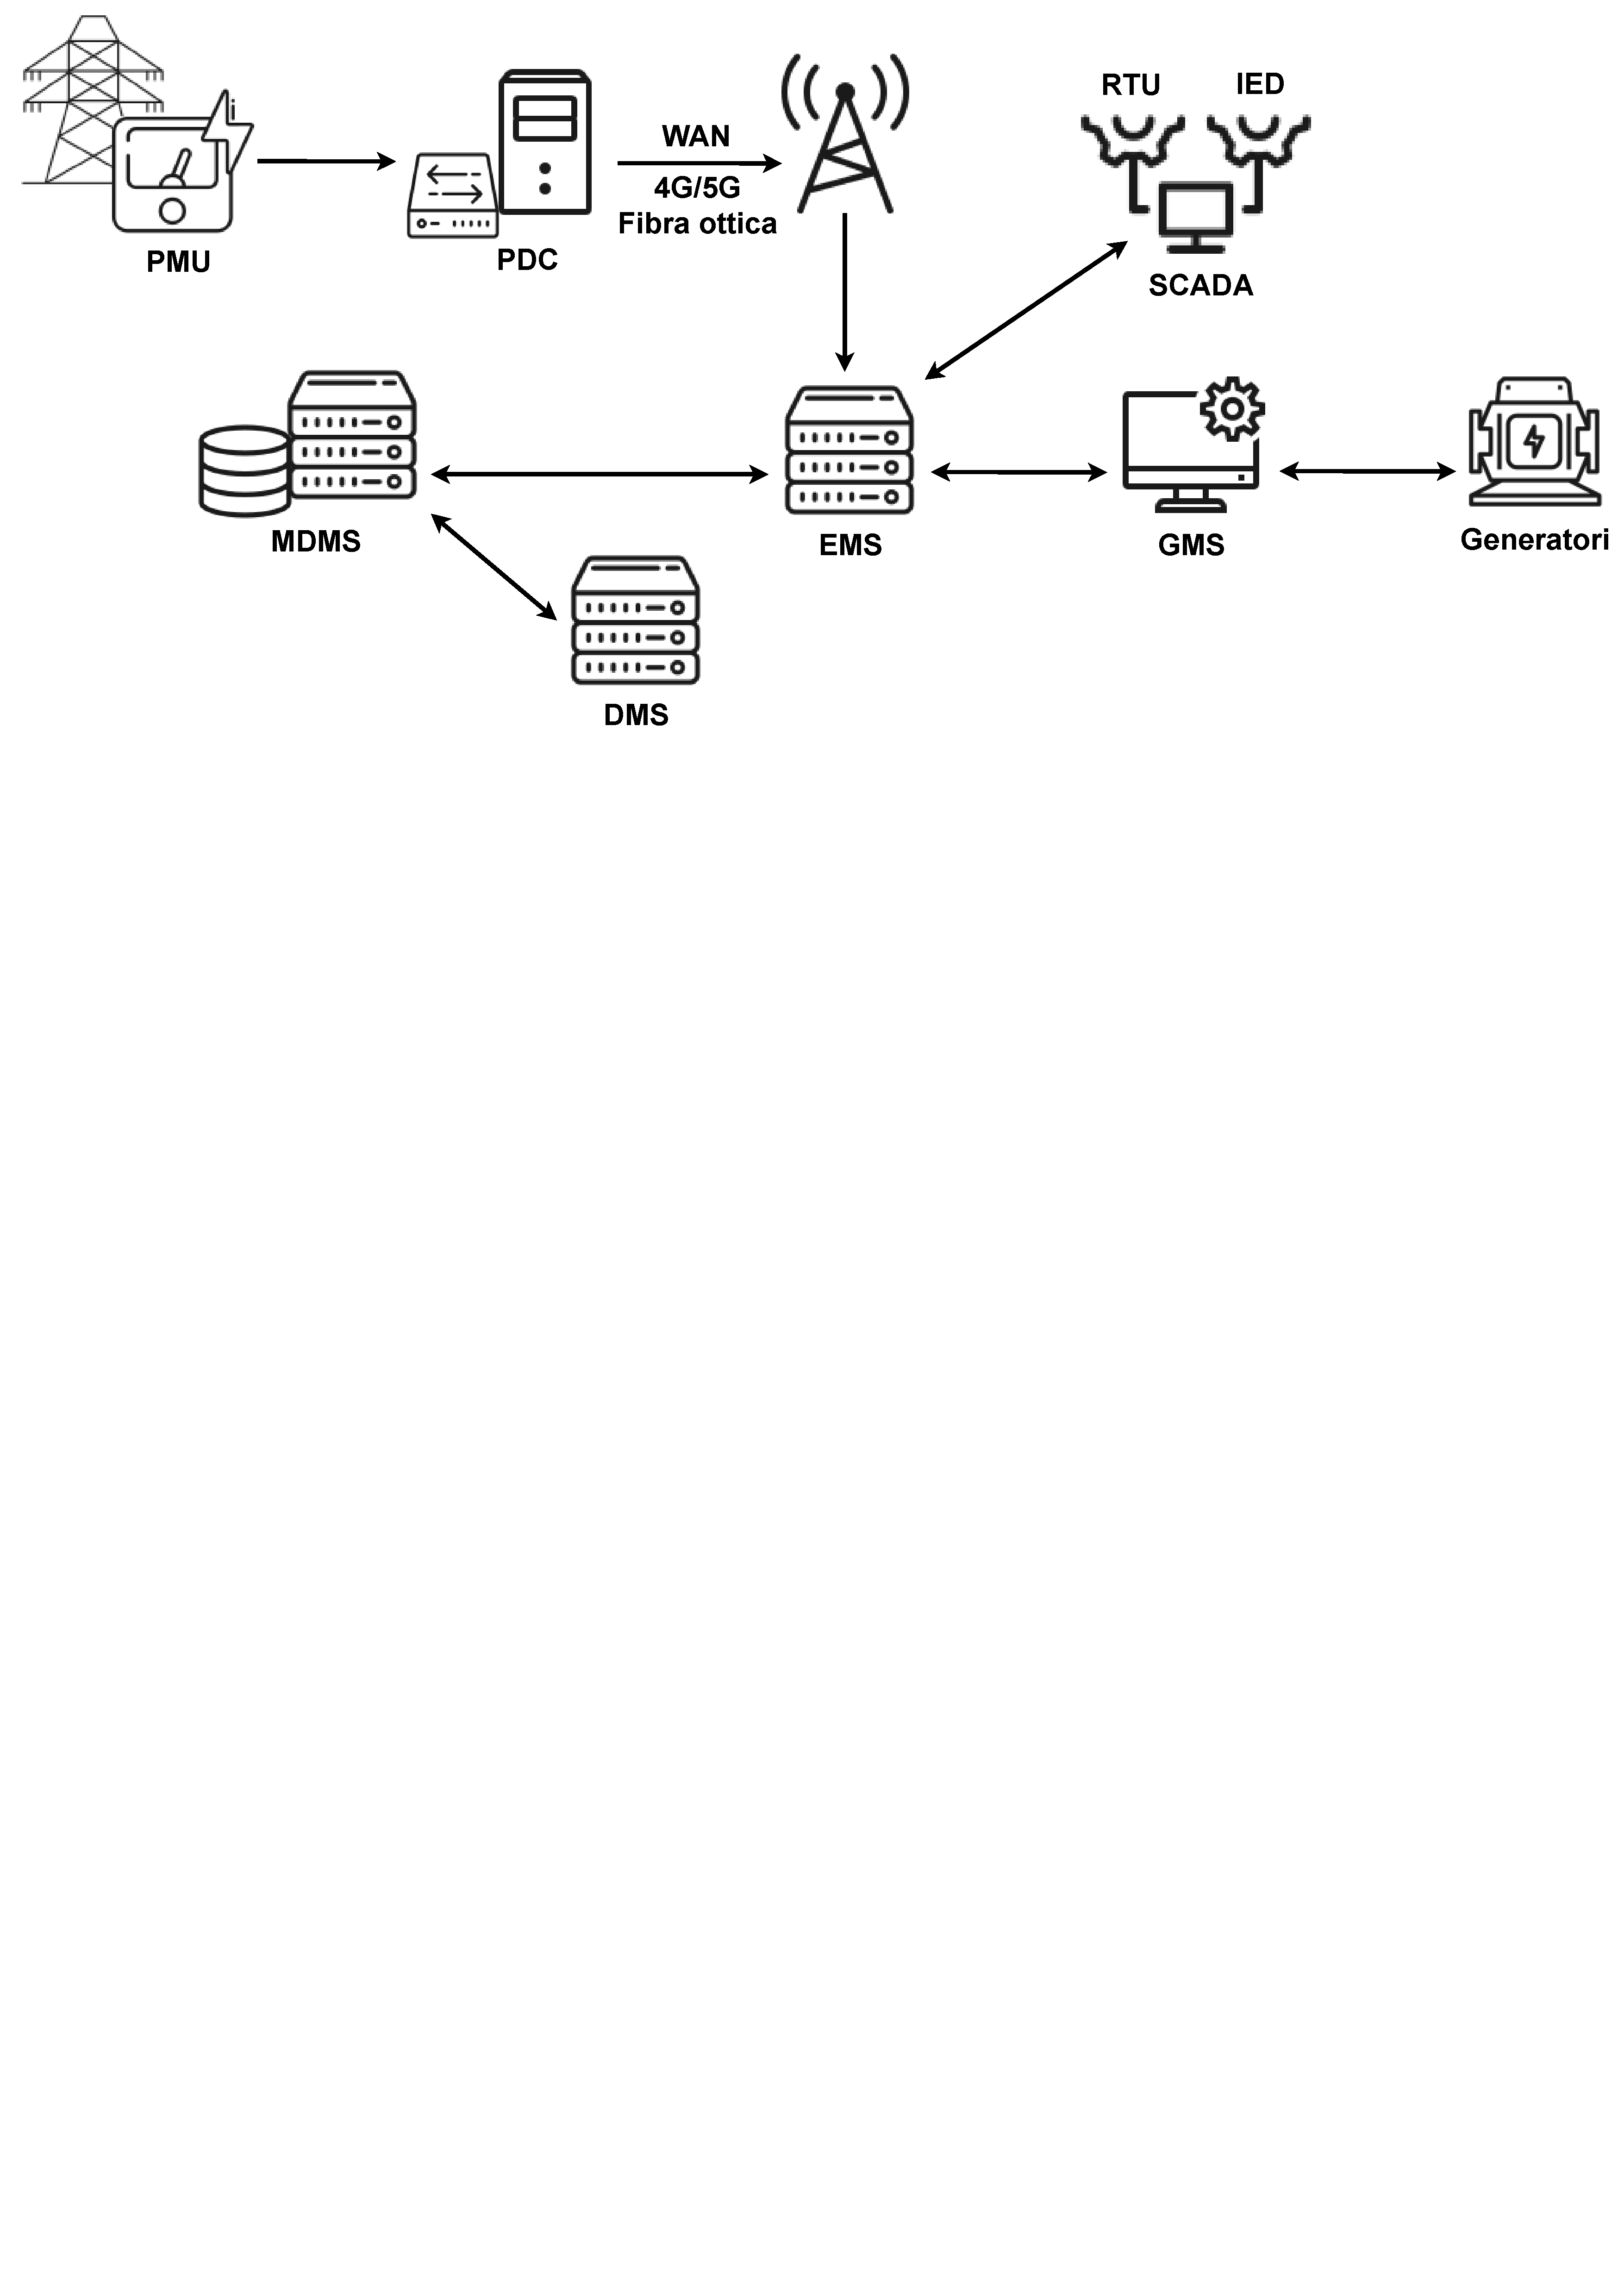
\includegraphics[trim= 0cm 57cm 0cm 0cm, clip, width=0.9\linewidth]{img/Operational-domain-v2.drawio.pdf}
    \caption{Dominio operazionale}
\end{figure}
